\documentclass[conference]{IEEEtran}
\usepackage{times}
\usepackage{graphicx}

% numbers option provides compact numerical references in the text. 
\usepackage[numbers]{natbib}
\usepackage{multicol}
\usepackage[bookmarks=true]{hyperref}

\usepackage{comment}
\usepackage{xspace}
\let\labelindent\relax %fixes error in enumitem created due to legacy reasons
\usepackage{enumitem}
\usepackage{amsmath,amssymb,amsfonts,amsthm}
\usepackage{algorithm,algorithmicx}
\usepackage[noend]{algpseudocode}
\algrenewcommand\algorithmicindent{0.5em} 
\usepackage{parskip}
%\usepackage{subfig}
\usepackage{subcaption}
\usepackage[dvipsnames]{xcolor}
% \usepackage{makecell}

\newtheorem{lemma}{Lemma}

\DeclareMathOperator*{\argmin}{arg\,min}
%\pdfinfo{
%   /Author (Homer Simpson)
%   /Title  (Robots: Our new overlords)
%   /CreationDate (D:20101201120000)
%   /Subject (Robots)
%   /Keywords (Robots;Overlords)
%}


\graphicspath{
	{./figs/}
}

\hypersetup{letterpaper,bookmarksopen,bookmarksnumbered,
pdfpagemode=UseOutlines,
colorlinks=true,
linkcolor=blue,
anchorcolor=blue,
citecolor=blue,
filecolor=blue,
menucolor=blue,
urlcolor=blue
}

% Caligraphic letters:
\newcommand{\calA}{\ensuremath{\mathcal{A}}\xspace}
\newcommand{\calC}{\ensuremath{\mathcal{C}}\xspace}
\newcommand{\calE}{\ensuremath{\mathcal{E}}\xspace}
\newcommand{\calG}{\ensuremath{\mathcal{G}}\xspace}
\newcommand{\calR}{\ensuremath{\mathcal{R}}\xspace}
\newcommand{\calM}{\ensuremath{\mathcal{M}}\xspace}
\newcommand{\calN}{\ensuremath{\mathcal{N}}\xspace}
\newcommand{\calX}{\ensuremath{\mathcal{X}}\xspace}
\newcommand{\calS}{\ensuremath{\mathcal{S}}\xspace}
\newcommand{\calQ}{\ensuremath{\mathcal{Q}}\xspace}
\newcommand{\calT}{\ensuremath{\mathcal{T}}\xspace}
\newcommand{\calL}{\ensuremath{\mathcal{L}}\xspace}
\newcommand{\calB}{\ensuremath{\mathcal{B}}\xspace}
\newcommand{\calW}{\ensuremath{\mathcal{W}}\xspace}
\newcommand{\calV}{\ensuremath{\mathcal{V}}\xspace}
\newcommand{\calP}{\ensuremath{\mathcal{P}}\xspace}
\newcommand{\calD}{\ensuremath{\mathcal{D}}\xspace}
\newcommand{\calF}{\ensuremath{\mathcal{F}}\xspace}
\newcommand{\calO}{\ensuremath{\mathcal{O}}\xspace}


% math
\newcommand{\R}{\mathbb{R}}
\newcommand{\Z}{\mathbb{Z}}
\newcommand{\A}{\mathbb{A}}
\newcommand{\N}{\mathbb{N}}
\newcommand{\Q}{\mathbb{Q}}
\newcommand{\C}{\mathbb{C}}
\newcommand{\K}{\mathbb{K}}

% Motion planning
\newcommand{\Cfree}{\ensuremath{\calX_{\rm free}}\xspace}
\newcommand{\Cforb}{\ensuremath{\calX_{\rm forb}}\xspace}
%\newcommand{\Csafe}{\ensuremath{\calX_{\rm free}^{\rm safe}}\xspace}
\newcommand{\Cspace}{\calC-space\xspace}

% =
\newcommand{\eg}{{e.g.,}\xspace}
\newcommand{\ie}{{i.e.,}\xspace}
\newcommand{\etc}{{etc.}\xspace}
\newcommand{\etal}{{et~al.}\xspace}

\def\naive{{na\"{\i}ve}\xspace}

\def\OS#1{\textcolor{magenta}{#1}}
\def\FI#1{\textcolor{cyan}{#1}}

\newtheorem{thm}{Theorem}
\newtheorem{lem}{Lemma}
%\newtheorem{thm}{Theorem}[section]
\newtheorem{observation}[thm]{Observation}
%\newtheorem{thm}{Theorem}
\newtheorem{cor}{Corollary}
\newtheorem{definition}[thm]{Definition}


%tex tools
\newcommand{\ignore}[1]{}
\newcommand{\first}[2]{#1}
\newcommand{\second}[2]{#2}
\newcommand{\arxiv}[2]{#2}


\newcommand\algname[1]{\textsf{#1}\xspace}
\newcommand\astar{\algname{A*}}


%paper-related macros
\newcommand\Gfull{\ensuremath{G^{\textrm{full}}}\xspace}
\newcommand\Shome{\ensuremath{s_{\textrm{home}}}\xspace}
\newcommand\Tbound{\ensuremath{t_{\textrm{bound}}}\xspace}
\newcommand\Trc{\ensuremath{t_{\textrm{rc}}}\xspace}
\newcommand\Ssc{\ensuremath{s_{\textrm{sc}}}\xspace}


%comments
\def\os#1{\textcolor{magenta}{#1}}
\begin{document}

% paper title
\title{Provably Constant-Time Planning and Re-planning for Real-time Grasping Objects off a Conveyor}

% You will get a Paper-ID when submitting a pdf file to the conference system
\author{Author Names Omitted for Anonymous Review. Paper-ID [1329]}

%\author{\authorblockN{Michael Shell}
%\authorblockA{School of Electrical and\\Computer Engineering\\
%Georgia Institute of Technology\\
%Atlanta, Georgia 30332--0250\\
%Email: mshell@ece.gatech.edu}
%\and
%\authorblockN{Homer Simpson}
%\authorblockA{Twentieth Century Fox\\
%Springfield, USA\\
%Email: homer@thesimpsons.com}
%\and
%\authorblockN{James Kirk\\ and Montgomery Scott}
%\authorblockA{Starfleet Academy\\
%San Francisco, California 96678-2391\\
%Telephone: (800) 555--1212\\
%Fax: (888) 555--1212}}


% avoiding spaces at the end of the author lines is not a problem with
% conference papers because we don't use \thanks or \IEEEmembership


% for over three affiliations, or if they all won't fit within the width
% of the page, use this alternative format:
% 
%\author{\authorblockN{Michael Shell\authorrefmark{1},
%Homer Simpson\authorrefmark{2},
%James Kirk\authorrefmark{3}, 
%Montgomery Scott\authorrefmark{3} and
%Eldon Tyrell\authorrefmark{4}}
%\authorblockA{\authorrefmark{1}School of Electrical and Computer Engineering\\
%Georgia Institute of Technology,
%Atlanta, Georgia 30332--0250\\ Email: mshell@ece.gatech.edu}
%\authorblockA{\authorrefmark{2}Twentieth Century Fox, Springfield, USA\\
%Email: homer@thesimpsons.com}
%\authorblockA{\authorrefmark{3}Starfleet Academy, San Francisco, California 96678-2391\\
%Telephone: (800) 555--1212, Fax: (888) 555--1212}
%\authorblockA{\authorrefmark{4}Tyrell Inc., 123 Replicant Street, Los Angeles, California 90210--4321}}


\maketitle

% \begin{abstract}
% Robots in warehouse environments typically perform repetitive tasks such as picking and placing of moving objects on a conveyor belt. Motion planning needs to be efficient and reliable in these domains to ensure high and consistent throughput. The success of manipulation tasks relies heavily on the accuracy of the perception system which often is noisy, especially if the target objects are perceived from a distance. For fast moving conveyor belts, the robot must start moving early on (relying on the first noisy estimate) to be able to reach the object in time and then adjust its motion as it gets improved estimates.
% To this end we propose a real-time replanning framework that would guarantee a bound on the reaction time of the robot whenever a perception update is received. Our key insight is that for repetitive tasks the paths look very similar and can efficiently be reused to minimise the processing time and memory footprint. Our framework leverages offline preprocessing to compute a representative set of paths (with some auxiliary data structures) which can then be used online to generate a plan from any point during execution (if one exists) in bounded time. We show our results on a 7 DOF robot arm, demonstrating the robot picking up objects from a conveyor belt.
% \end{abstract}

\begin{abstract}
In warehousing and manufacturing environments, manipulation platforms are frequently deployed at conveyor belts to perform pick and place tasks. Because objects on the conveyor belts are moving, robots have limited time to pick them up. This brings the requirement for fast and reliable motion planners that could provide provable real-time planning guarantees, which the existing algorithms do not provide. Besides the planning efficiency, the success of manipulation tasks relies heavily on the accuracy of the perception system which often is noisy, especially if the target objects are perceived from a distance. For fast moving conveyor belts, the robot cannot wait for a perfect estimate before it starts execution. In order to be able to reach the object in time it must start moving early on (relying on the initial noisy estimates) and adjust its motion on-the-fly in response to the pose updates from perception. We propose an approach that meets these requirements by providing provable constant-time planning and replanning guarantees. We present it, give its analytical properties and show experimental analysis in simulation and on a real robot.
\end{abstract}


\IEEEpeerreviewmaketitle

\section{Introduction}
%1. What is the problem?
%2. Why is it relevant?
%3. Why is it hard?
%4. What have others done?
%5. What's missing?
%6. What is our ONE key insight?
%7. How do we compare against the state of the art?
%8. What are our contributions?
%9. What are our limitations?

%% motivation
Conveyor belts are widely used in automated distribution, warehousing, as well as for manufacturing and production facilities. In the modern times robotic manipulators are being deployed extensively at the conveyor belts for automation and faster operations~\cite{zhang2018gilbreth}. In order to maintain a high-distribution throughput, manipulators must pick up moving objects without having to stop the conveyor for every grasp. In this work, we consider the problem of motion planning for grasping moving objects off a conveyor. An object in motion imposes a requirement that it should be picked up in a short window of time. The motion planner for the arm, therefore, must compute a path within a bounded time frame to be able to successfully perform this task.


%% why replanning?
    Manipulation relies on high quality detection and localization of moving objects. When the object first enters the field of view of the robot, the initial perception estimates of the object's pose are often inaccurate. Consider the example of an object (sugar box) moving along the conveyor towards the robot in Fig.~\ref{fig:intro_pic}, shown through an image sequence as captured by the robot's Kinect camera in Fig.~\ref{fig:pose_sequence}. In order to understand how pose estimation error varies as the object gets closer, we filter the input point cloud and remove all points lying outside the conveyor. We then compute the pair-wise minimum distance between the input point cloud and a predicted point cloud that corresponds to the object's 3D model transformed with the predicted pose through ICP~\cite{besl1992method} refinement. The plot in Fig.~\ref{fig:pose_sequence} shows the variation of the average pairwise minimum distance between the two point clouds as the object gets closer. We can observe that the distance decreases as the object moves closer, indicating that the point clouds overlap more closely due to more accurate pose estimates closer to the camera.
    
% The black color denotes points corresponding to the object in the observed scene after filtering out all points lying outside the conveyor. The white point cloud shows the object's 3D model transformed with the predicted 3-Degree of Freedom pose obtained by using Iterative Closest Point (ICP)~\cite{besl1992method} refinement. Upon observation of the overlap between the point clouds, we see that they begin to overlap more closely as the object moves towards the robot, indicating that the pose estimate is becoming increasingly accurate. 
However, if the robot waits too long to get an accurate estimate of the object pose, the delay in starting plan execution could cause the robot to miss the object. The likelihood of this occurring increases proportionately with the speed of the conveyor. Therefore, the robot should start executing a plan computed for the initial pose and as it gets better estimates, it should repeatedly replan for the new goals. However, for every replanning query, the time window for the pickup shrinks. This makes the planner's job difficult to support real-time planning.

\begin{figure}[t]
    \centering
    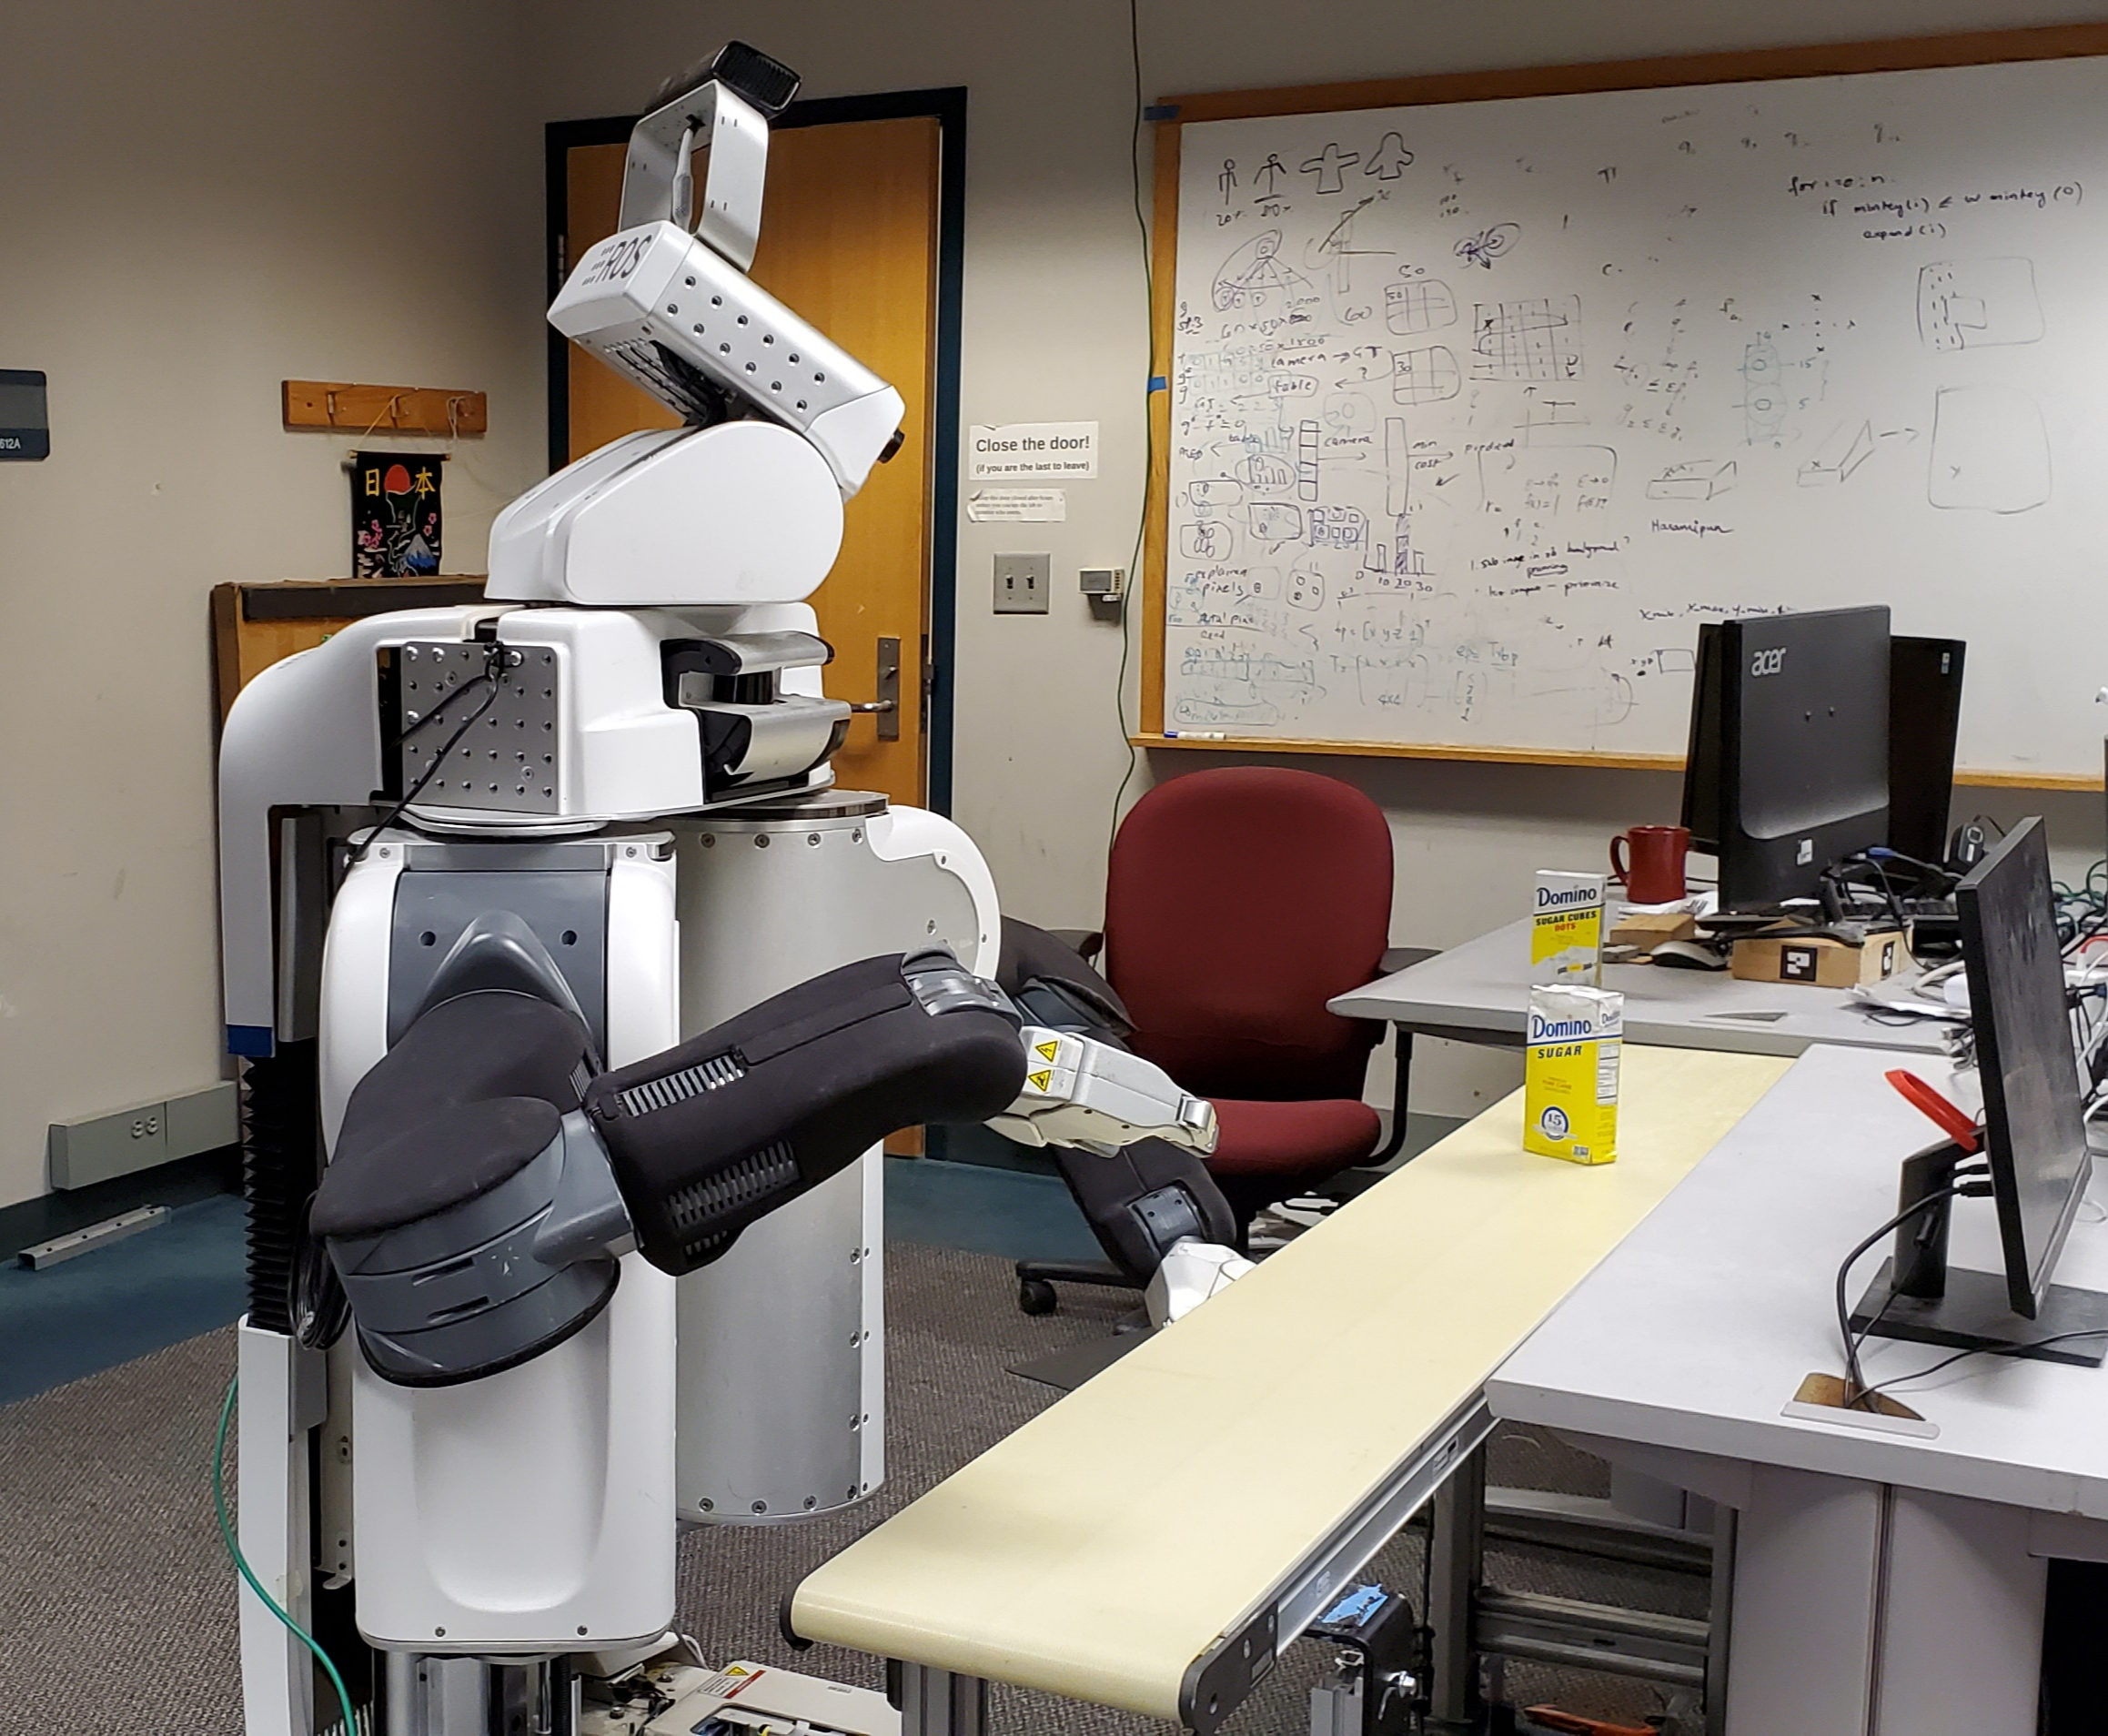
\includegraphics[width=0.25\textwidth]{figs/cover_pic.jpg}
    \caption{
    \CaptionTextSize
    A scene demonstrating the PR2 robot picking up a moving object (sugar box) off a conveyor belt.}
    \label{fig:intro_pic}
    \vspace{-7.5mm}
\end{figure}


%% why problem is hard
Furthermore, the planning problem is challenging because the motion planner has to account for the dynamic object and thus plan with time as one of the planning dimension. It should generate a valid trajectory that avoids collision with the environment around it and also with the target object to ensure that it does not damage or topple it during the grasp. Avoiding collisions with the object requires precise geometric collision checking between the object geometry and the geometry of the manipulator. The resulting complexity of the planning problem makes it infeasible to plan online for this task.

%%
Motivated by these challenges, we propose a planning framework that leverages offline preprocessing to provide bounds on the planning time when the planner is invoked online. Our key insight is that in our domain the manipulation task is highly repetitive---even for different object poses, the computed paths are quite similar and can be efficiently reused to speed up online planning. Based on this insight, we derive a method that precomputes a representative set of paths offline with some auxiliary datastructures and uses them online to plan in constant time. Here, we assume that the models of the target objects are known. Namely, the planner is provided with the geometric model of the target object apriori. To the best of our knowledge, our approach is the first to provide provable constant-time planning guarantees on generating motions all the way to the goal for dynamic environments.

%
We experimentally show that constant-time planning and replanning capability is necessary for a successful conveyor pickup task. Specifically if we only perform one-time planning, (namely, either following the plan for the initial noisy pose estimate or from a delayed but accurate pose estimate) we frequently fail to pick the object.
\begin{figure}[t]
    \centering
    \begin{subfigure}{.225\textwidth}
    %   \centering
        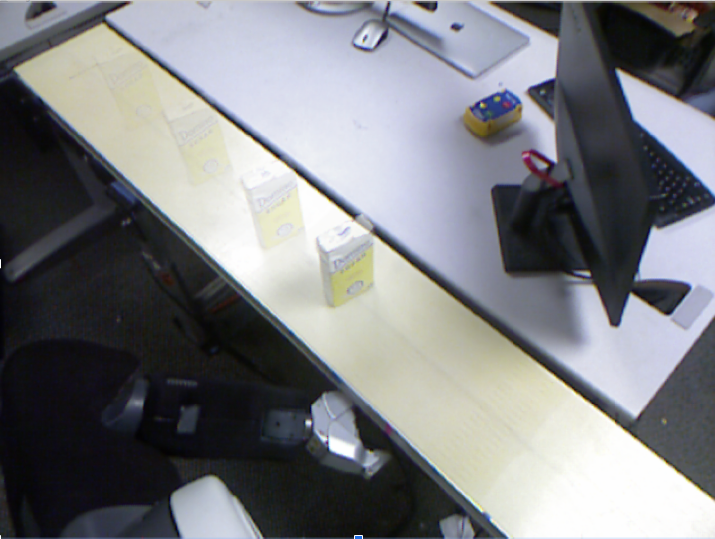
\includegraphics[width=0.9\textwidth]{object_blur}
        \caption{}
        \label{fig:obj1}
    \end{subfigure}
    \begin{subfigure}{0.225\textwidth}
    %   \centering
        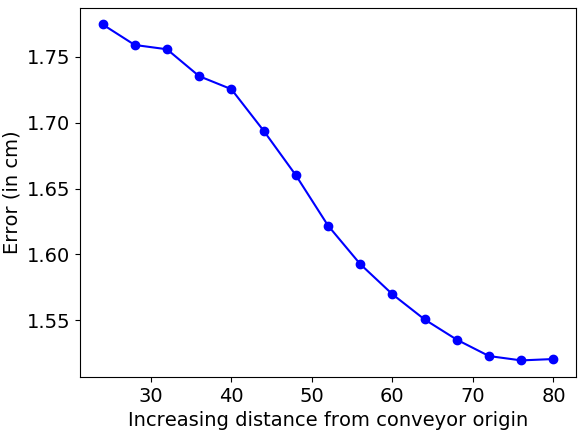
\includegraphics[width=0.9\textwidth]{pose_error_f}
        \caption{}
        \label{fig:obj2}
    \end{subfigure}
    \caption{
    \CaptionTextSize
    (\subref{fig:obj1})~Depiction of an object moving along a conveyor towards the robot.
    %
    (\subref{fig:obj2})~Pose error as a function of the distance from the conveyor's start.
    %, calculated as the average pair wise minimum distance between the input point cloud and the point cloud corresponding to the predicted pose.
    }
    \label{fig:pose_sequence}
    \vspace{-7.5mm}
\end{figure}

\section{Related work}
\subsection{Motion planning for conveyor pickup task}
Existing work on picking moving objects has focused on different aspects of the problem ranging from closed-loop controls to object perception and pose estimation, motion planning and others~\cite{allen1993automated, han2019toward, stogl2017tracking, zhang2018gilbreth}. 
%
Here, we focus on motion-planning related work. Graph-searched based approaches have been used for the motion-planning problem~\cite{cowley2013perception, menon2014motion}. The former uses a kinodynamic motion planner to smoothly pick up moving objects i.e., without an impactful contact. A heuristic search-based motion planner that plans with dynamics and could generate optimal trajectories with respect to the time of execution was used. While this planner provides strong optimality guarantees, it is not real-time and thus cannot be used online.
%
The latter work was demonstrated in the real world showing real-time planning capability. While the planner is fast, it does  pure kinematic planning and does not require collision checking with the target object. The approach plans to a pregrasp pose and relies on Cartesian-space controllers to perform the pick up. The usage of the Cartesian controller limits the types of objects that the robot can grasp.


\subsection{Preprocessing-based planning}
Preprocessing-based motion planners often prove beneficial for real-time planning. They analyse the configuration space offline to generate some auxiliary information that can be used online to speed up planning. 
Probably the best-known example is the Probablistic Roadmap Method (\algname{PRM})~\cite{kavraki1996probabilistic} which precomputes a roadmap that can answer any query by connecting the start and goal configurations to the roadmap and then searching the roadmap. \textsf{PRM}s are fast to query yet they do not provide constant-time guarantees.
Moreover for a moving object (as we have in our setting), they would require edge re-evaluation which is often computationally expensive.
%

A provably constant-time planner was recently proposed in~\cite{islam2019planning}. Given a start state and a goal region, it precomputes a compressed set of paths that can be utilised online to plan to any goal state within the goal region in bounded time. As we will see, our approach bears close resemblance with this work in the context of the paths-compression mechanism.
%

Using either of these two methods (\cite{islam2019planning,kavraki1996probabilistic}) in our context is not straightforward as they are only applicable to pure kinematic planning and thus they cannot be used for the conveyor-planning problem.
%

Another family of preprocessing-based planners utilises previous experiences to speed up the search~\cite{BAG12,CSMOC15,PCCL12}. Experience graphs~\cite{PCCL12}, provide speed up in planning times for repetitive tasks by trying to reuse previous experiences. These methods are also augmented with sparsification techniques (see e.g.,~\cite{DB14,SSAH14}) to reduce the memory footprint of the algorithm.
Unfortunately, none of the mentioned algorithms provide bounded planning-time guarantees that are required by our application.

\subsection{Online replanning and real time planning}
The conveyor-planning problem can be modelled as a Moving Target Search problem (MTS) which is a widely-studied topic in the graph search-based planning literature~\cite{ishida1991moving,ishida1995moving,koenig2007speeding,sun2010moving}. 
These approaches interleave planning and execution incrementally and update the heuristic values of the state space to improve the distance estimates to the moving target. Unfortunately, in high-dimensional planning problems, this process is computationally expensive which is why these approaches are typically used for two-dimensional grid problem such as those encountered in video games.

Similar to MTS, real-time planning was widely considered in the search community (see, e.g.,~\cite{KL06,KS09,korf1990real}).
However, as mentioned, these works are typically applicable to low-dimensional search spaces.
%
Finally it is worth mentioning that some finite-time properties have been obtained for sampling-based planners~\cite{JansonIP18} but these come in form of big-$O$ notation, thus they are not applicable to our setting, when we are aiming for tight planning times (e.g., less than one second).


\section{Problem definition}
Our system is comprised of 
a robot manipulator~$\calR$,
a conveyor belt~$\calB$ moving at some known velocity,
a set of known objects~$\calO$ that need to be grasped and 
a perception system~$\calP$ that is able to estimate the type of object and its location on~$\calB$.

Given a pose $g$ of an object $o \in \calO$, our task is to plan the motion of $\calR$ such that it will be able to pick~$o$ from~$\calB$ at some future time.
%
Unfortunately, the perception system $\calP$ may give inaccurate object poses.
Thus, the pose $g$ will be updated by~$\calP$ as $\calR$ is executing its motion. 
To allow for $\calR$ to move towards the updated pose in real time, we introduce the additional requirement that planning should be done within a predefined time bound~\Tbound.
%
For ease of exposition, when we say that we plan to a pose $g$ of $o$ that is given by $\calP$, 
we mean that we plan the motion of $\calR$ such that it will be able to pick~$o$ from~$\calB$ at some future time. 
This is explained in detail in Sec.~\ref{sec:eval} and in Fig.~\ref{fig:pe}.

%
We denote by $\Gfull$ the discrete set of initial object poses on $\calB$ that $\calP$ can perceive.
%
Finally, we assume that $\calR$ has an initial configuration \Shome from which it will start its motion to grasp any object.


Roughly speaking, the objective, following the set of assumptions we will shortly state, is to enable planning to any goal pose $ g \in \Gfull$ in bounded time~\Tbound regardless of $\calR$'s current configuration.
%More specifically, the perception system is setup such that it sends updated pose estimates on the fly as the object moves along the conveyor belt and as the robot approaches the object.   
To formalize this idea, let us introduce the notion of a \emph{reachable} state:

\begin{definition}
    A goal pose $g \in \Gfull$ is said to be \emph{reachable} from a state $s$ if there exists a path from $s$ to $g$ and it can be computed in finite time.
\end{definition}

Given a state $s$ we denote the set of all goals that are reachable from $s$ as $G^{\rm reach}(s)$ and we say that $G^{\rm reach}(s)$ is \emph{reachable} from $s$.

\begin{definition}
    A reachable pose $g \in \Gfull$ is said to be \emph{covered} by a state $s$ if 
    the system can plan a path from $s$ to $g$ within time~\Tbound.
\end{definition}

Thus, we wish to build a system such that 
for any state $s$ that the system can be in 
and every reachable goal pose $g \in \Gfull$ updated by~$\calP$,
$g$ is covered by $s$.


We are now ready to state the assumptions for which we can solve the problem defined.
%\begin{definition}
%    A goal region $G \subseteq \Gfull$ is said to be \emph{reachable} from a state $s$ if any state $g \in G$ is reachable from $s$.
%\end{definition}

We make the following assumptions about the system.
\begin{enumerate}[label={\textbf{A\arabic*}},leftmargin=0.75cm]
    % \item \label{assum:1} The goal set \Gfull is reachable from the start state~\Shome. Namely,  $G^{\rm reach}(\Shome) = \Gfull$.
    
\ignore{
    \item \label{assum:2} Given a path 
    $\Pi = \{s_0, \ldots, s_k \}$ 
    s.t. $s_0 = \Shome$ and $s_k \in \Gfull$, 
    we have that $G^{\rm reach}(s_{i+1}) \subset G^{\rm reach}(s_{i})$.
    Namely, the reachable set of goals for a state on the path is a subset of the reachable set of every other state on that path that exists before it.
    \os{Oren - Didn't we agree that this is not an assumption but a property?}
}

%    \item \label{assum:3} \Gfull would accommodate for an error $\epsilon$ in the initial pose estimate $g_{\textrm{init}}$ of the perception system. Each subsequent estimate $g_{\textrm{next}}$ will be within the $\epsilon$ window around $g_{\textrm{init}}$ (in retrospect because the conveyor is moving).
 
    \item \label{assum:4} There exists a replan cutoff time \Trc from when the robot starts moving, after which the planner does not replan and continues to execute the last planned path.

    \item \label{assum:5} If the robot starts moving at $t = 0$ then for any time $t < \Trc$, the environment is static. Namely, objects on~$\calB$ cannot collide with $\calR$ during that time.
    
    \item \label{assum:3} Given an initial goal pose $g_{\textrm{init}} \in \Gfull$ by $\calP$, any subsequent pose $g_{\textrm{new}} \in \Gfull$ is at most $\varepsilon_\calP$ distance away from $g_{\textrm{init}}$ (after accounting for the fact that the object moved along $\calB$).
    

\end{enumerate}

Assumptions~\ref{assum:4}-\ref{assum:5} enforce a requirement that $\calP$ must provide an accurate estimate $g$ while $o$ is at a safe distance from $\calR$.
%
Assumption~\ref{assum:3} corresponds to the error tolerance of the perception system. This is explained in detail in Sec.~\ref{sec:eval} and in Fig.~\ref{fig:pe}
% Assumption~\ref{assum:1} corresponds to properties of the environment \emph{without} taking the objects on the conveyor belt into account 
% while


% Assumptions~\ref{assum:3}-\ref{assum:5} correspond to properties of the environment that account for the perception system and the objects on the conveyor belt.


\section{Algorithmic framework}
\label{subsec:strawman}
Our approach for bounded-time planning relies on a \emph{preprocessing} stage that allows to efficiently compute paths in a \emph{query} stage to any goal state (under Assumptions~\ref{assum:4}-\ref{assum:3}). 
%
Before we describe our approach, we start by describing a \naive method that solves the aforementioned problem but requires a prohibitive amount of memory.
%
This can be seen as a warmup before describing our algorithm which exhibits the same traits but doing so in a memory-efficient manner.

\subsection{Straw man approach}
\begin{figure}[t]
    \centering
    \begin{subfigure}{.225\textwidth}
    %   \centering
        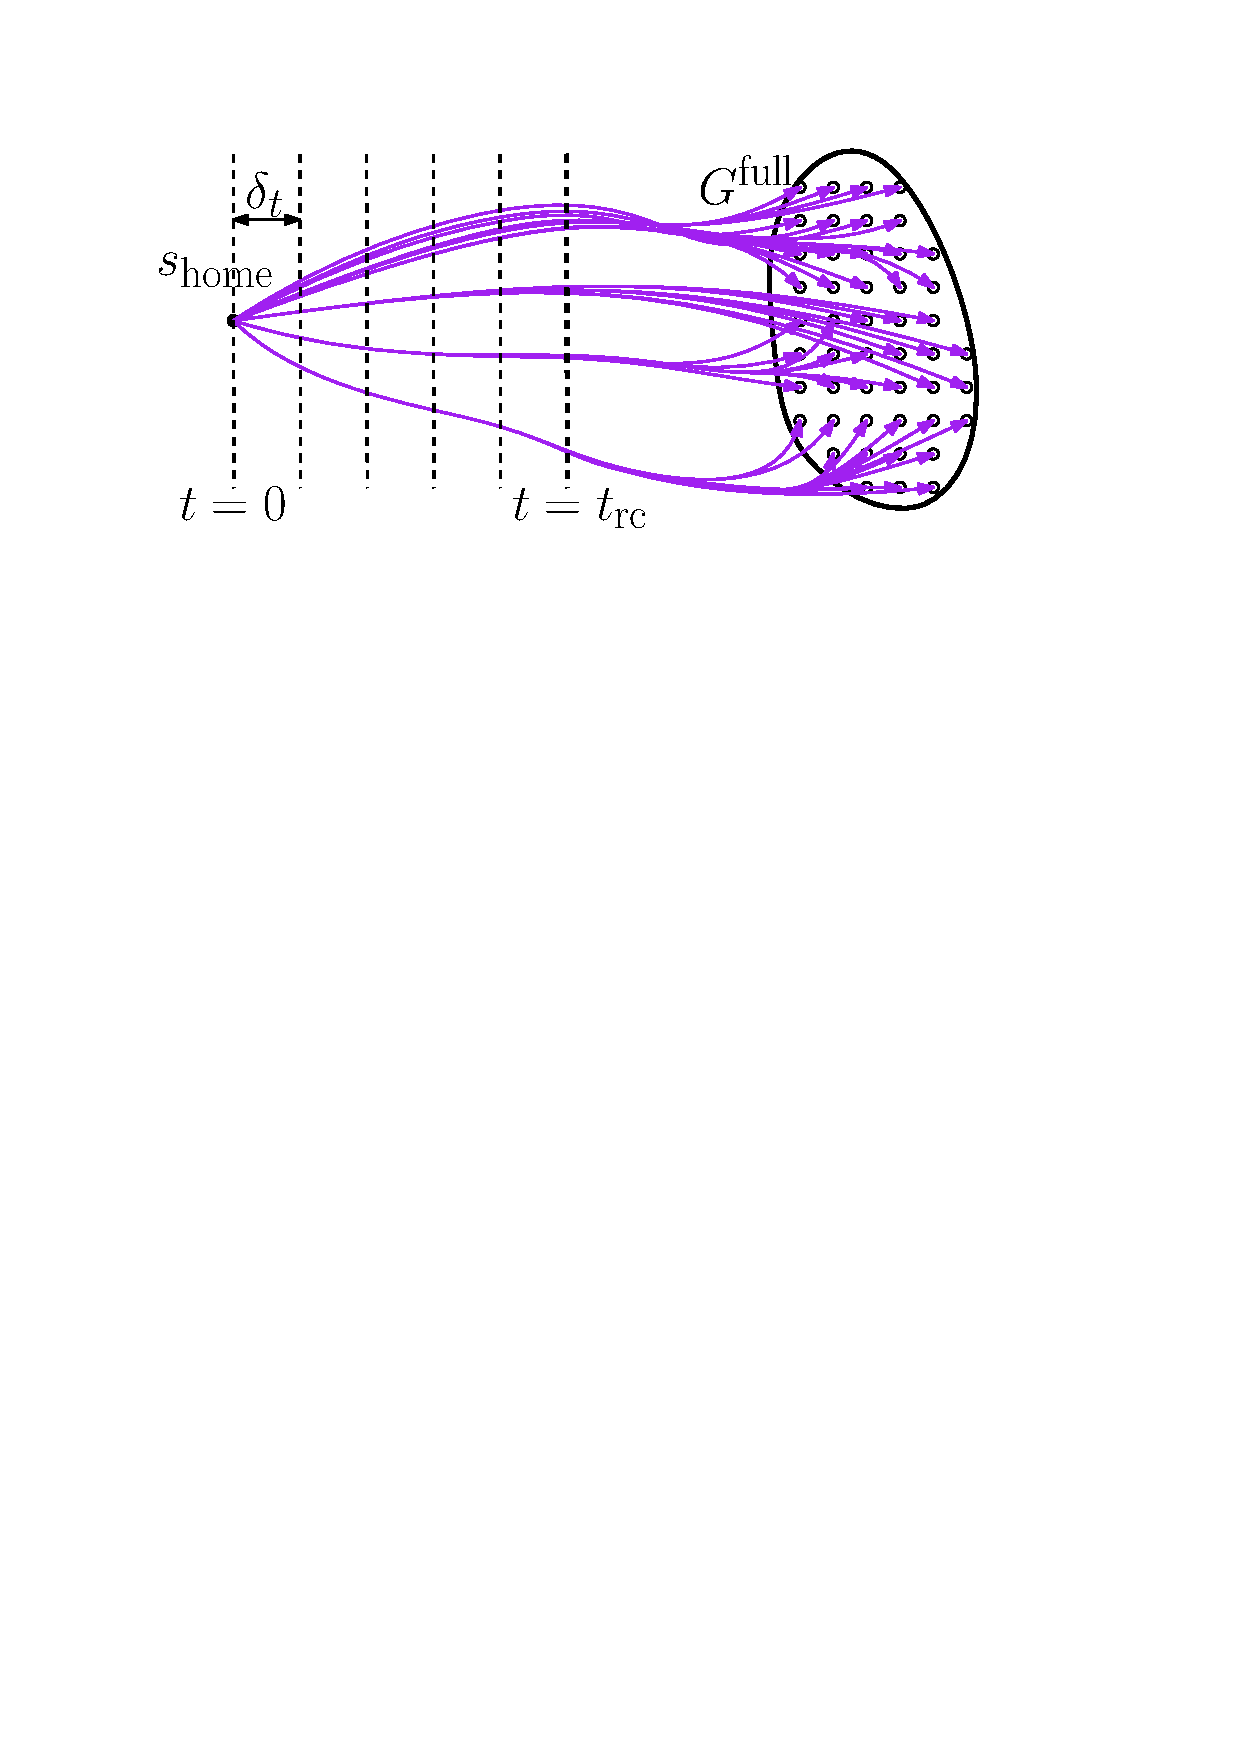
\includegraphics[width=0.9\textwidth]{naive1}
        \caption{}
        \label{fig:naive1}
    \end{subfigure}
    \hfill
    \begin{subfigure}{0.225\textwidth}
    %   \centering
        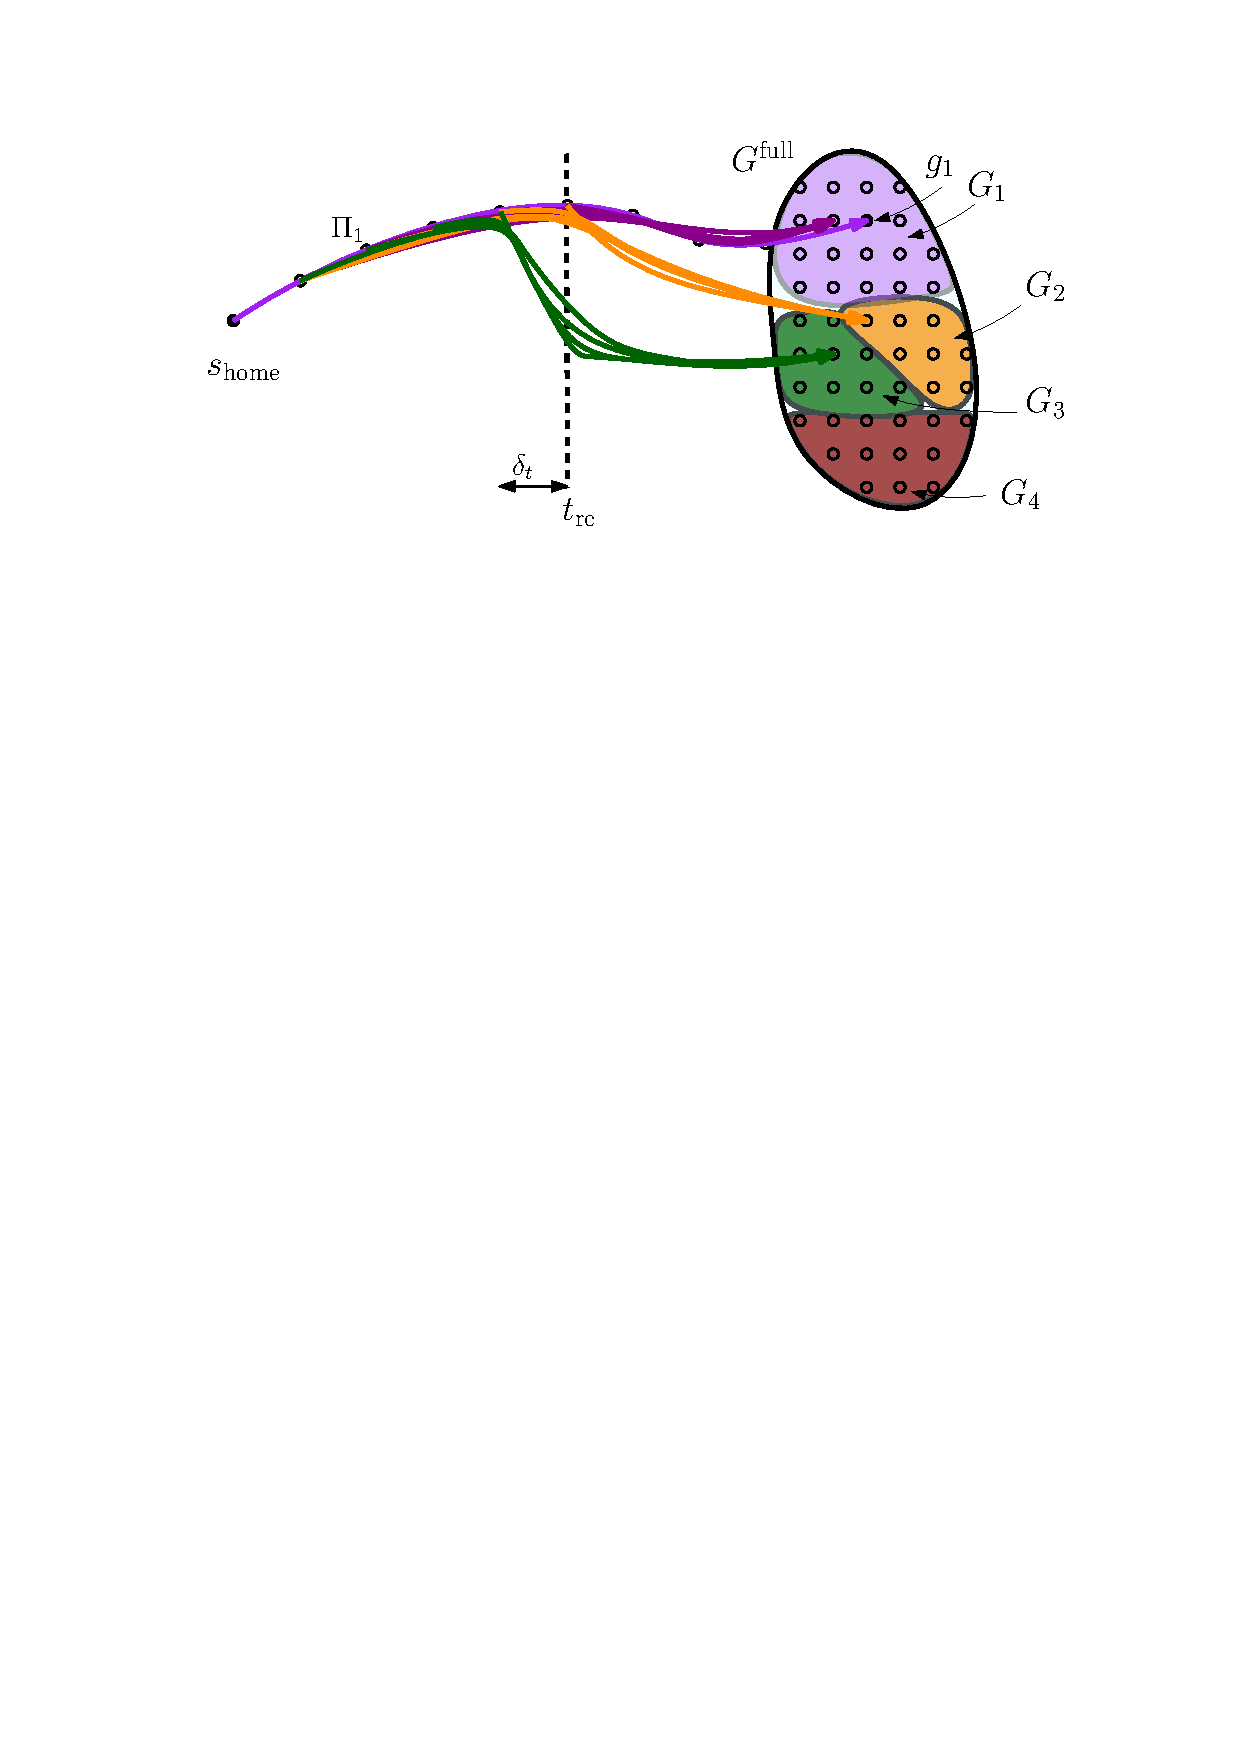
\includegraphics[width=0.9\textwidth]{naive2}
        \caption{}
        \label{fig:naive2}
    \end{subfigure}
    \caption{
    \CaptionTextSize
    The two steps of the preprocessing stage of the straw man algorithm. In both figures, paths that are very similar (and their corresponding goal states) are depicted using the same color.
    (\subref{fig:naive1})~First step---the algorithm computes a path from \Shome to every state in \Gfull.
    %
    (\subref{fig:naive2})~Second step---the algorithm computes for each path a new path to each goal state for every state along the path. Here, one representative path is depicted together with three different goal states. 
    This is repeated recursively for the new paths but not visualized.}
    \label{fig:naive}
    \vspace{-5mm}
\end{figure}

We divide the preprocessing stage into two steps.
In the first step, we compute from \Shome a path $\Pi_g$ to every reachable $g \in \Gfull$. 
%(such a path exists following \ref{assum:1}).
. Thus, all goal states are covered by \Shome and this allows us to start executing a path once $\calP$ gives its initial pose estimate.
However, we need to allow for updated pose estimations while executing~$\Pi_g$. 

%
Following \ref{assum:4} and \ref{assum:5}, this only needs to be done up until time~\Trc.
Thus, we discretize each path such that consecutive states along the path are no more than $\delta _t$ time apart. As we will see, this will allow the system to start executing a new path within $\Tbound + \delta_t$ after a new pose estimation is obtained from $\calP$.
%
We call all states that are less than \Trc time from \Shome \emph{replanable states}.


In the second step of the preprocessing stage, for every replanable state along each path $\Pi_g$, we compute a new path to all goal states. 
%\bound{that are $\varepsilon_\calP$ away from $g$}.
See Fig.~\ref{fig:naive}.
%
This will ensure that all goal states are covered by the replanabale states that were introduced in the first step of the preprocessing stage. Namely, it will allow to immediately start executing a new path once the goal location is updated by~$\calP$.
%
Unfortunately,~$\calP$ may update the goal location more than once. Thus, this process needs to be performed recursively for the new paths as well.


The outcome of the preprocessing stage is a set of precomputed collision-free paths starting at states that are at most $\Trc$ from \Shome and end at goal states.
The paths are stored in a lookup table that can be queried in $O(1) < \Tbound$ time.

In the query stage we obtain an estimation $g_1$ of the goal pose by $\calP$. 
The algorithm then retrieves the path~$\Pi_1(\Shome,g_1)$ from~\Shome to~$g_1$ and the robot starts executing~$\Pi_1(\Shome,g_1)$.
%
For every new estimation $g_i$ of the goal pose obtained from~$\calP$  while the system is executing path $\Pi_{i-1}(s,g_{i-1})$, the algorithm retrieves from the lookup table the path $\Pi_i(s',g_i)$ from the first state~$s'$ along $\Pi_{i-1}(s,g_{i-1})$ that is $\Tbound + \delta_t$ time from~$s$. The robot~$\calR$ will then start executing~$\Pi_i(s',g_i)$ once it reaches~$s'$.

Clearly, every state is covered by this brute-force approach, however it requires a massive amount of memory.
Let $n_{\rm goal} = \vert \Gfull \vert$ be the number of goal states and
$\ell$ be the number of states between \Shome and the state that is \Trc time away.
This approach requires precomputing and storing $O(n_{\rm goal}^\ell)$ paths which is clearly infeasible.
In the next sections, we show how we can dramatically reduce the memory footprint of the approach without compromising on the system's capabilities.




\subsection{Algorithmic approach}
While the straw man algorithm presented  allows for planning to any goal pose $ g \in \Gfull$ in bounded time~\Tbound, its memory footprint is prohibitively large.
%
We suggest to reduce the memory footprint by building on the observation that many paths to close-by goals traverse very similar parts of the configurations space (see Fig.~\ref{fig:naive}).

Similar to the straw man algorithm, our preprocessing stage runs in two steps.
In the first step we  compute from \Shome a path $\Pi_g$ to every goal state $ g \in \Gfull$. However, this is done by computing a set of so-called ``root paths'' $\{\Pi_1, \ldots, \Pi_k \}$ from \Shome to a subset of goals in \Gfull (here we will have that $k \ll n_{\rm goal})$. 
As we will see, these paths will allow to efficiently compute paths to every goal state in the query stage and the system only needs to explicitly store these root paths in memory (and not a path to every goal state as in the straw man algorithm).
%
In the second step of the preprocessing stage, the algorithm recursively computes for all replanabale states along all root paths a new path to each goal state. However, this is done by attempting to re-use previously-computed root paths which, in turn, allows for a very low memory footprint.
%
It is important to note that replanable states are not only the ones that lie on the root paths from \Shome---whenever the recursion happens we compute a new set of root paths and generate new replanable states
%
The remainder of this section formalizes these ideas.

\subsection{Algorithmic building blocks}
We start by introducing the algorithmic building blocks that we use.
Specifically, we start by describing the motion planner that is used to compute the root paths 
and then continue to describe how they can be used as \emph{experiences} to efficiently compute paths to near-by goals.
\subsubsection{Motion planner}
We use a heuristic search-based planning approach with motion primitives (see, e.g,~\cite{CCL10,CSCL11,LF09})
as it allows for deterministic planning time which is key in our domain.
Moreover, such planners can easily handle under-defined goals as we have in our setting---we define a goal as a six DoF grasp pose for the goal object while our robot has seven DoFs and we need to acount for the grasping time.

\textbf{State space and graph construction.}
We define a state $s$ as a pair $(q,t)$ where $q = (\theta_1, ..., \theta_n)$ is a configuration represented by the joint angles for an $n$-DOF robot arm (in our setting $n=7$) and $t$ is the time associated with $q$.
%
Given a state $s$ we define two types of motion primitives which are short kinodynamically feasible motions that the robot~$\calR$ can execute. The first, which we term \emph{predefined} primitives are used to move to a pre-grasp position while the second, termed \emph{dynamic} primitives are used to perform grasping after the robot reached a pre-grasp position.
%

The predefined primitives are small individual joint movements in either direction as well as wait actions.
For each motion primitive, we compute its duration by using a nominal constant velocity profile for the  joint that is moved.
%\footnote{Computing a plan using these motion primitives is not guaranteed to respect the acceleration limits of $\calR$. However, in practice this seldom occurs and we elaborate in Sec.~\ref{sec:eval} how we handle these execution errors.}.
%

The dynamic primitives are generated by using a Jacobian pseudo inverse-based control law similar to what~\cite{menon2014motion} uses. 
The velocity of the end effector is computed such that the end-effector minimizes the distance to the grasp pose. Once the gripper encloses the object, it moves along with the object until the gripper is closed.
Additional details omitted due to lack of space. 

\textbf{Motion planner.}
The states and the transitions implicitly define a graph $\calG = (S,E)$ where $S$ is the set of all states and~$E$ is the set of all transitions defined by the motion primitives. We use Weighted \astar (\wastar)~\cite{pohl1970heuristic} to find a path in $\calG$ from a given state~$s$ to a goal state $g$. 
\wastar is a suboptimal heursitic search algorithm that allows a tradeoff between optimality and greediness by inflating the heuristic function by a given weight~$w$. 
The search is guided by an efficient and fast-to-compute heuristic function which in our case has two components.
The first component drives the search to intercept the object at the right time and 
the second component guides the search to correct the orientation of the end effector as it approaches the object. 
More formally, our heuristic function is given by
\vspace{-3mm}
$$
 h(s,g) = \max (w \cdot t(s,g), \textsc{AngleDiff}(s,g)).
$$
Here, $t(s,g)$ is the expected time to intercept the object which can be analytically computed from the velocities and positions of the target object and the end-effector and \textsc{AngleDiff}($s,g$) gives the magnitude of angular difference between the end-effector's current pose and target pose.

\subsubsection{Planning using experiences}
We now show how previously computed paths which we call ``experiences" can be reused in our framework. Given a heuristic function $h$ we define for each root path $\Pi$ and each goal state $g \in \Gfull$ the \emph{shortcut} state $\Ssc (\Pi,g)$ as the  state that is closest to~$g$ with respect~$h$.
Namely,
\vspace{-3mm}
$$
\Ssc (\Pi,g) := \argmin\limits_{s_i \in \Pi} h(s_i, g).
$$
Now, when searching for a path to a goal state $g \in \Gfull$ we add $\Ssc (\Pi,g)$ as a successor for any state along $\Pi$
(subject to the constraint that the path along $\Pi$ to \Ssc is collision free). In this manner we reuse previous experience to quickly reach a state close to the $g$.

\ignore{
\subsubsection{Planning using experiences}
We now show how \emph{experience graphs}~\cite{PCCL12} can be used in our framework.
%
Roughly speaking, experience graphs allow a planner  to accelerate its planning efforts whenever possible by using previously-computed paths. The planner gracefully degenerates to planning from scratch if no previous planning experiences can be reused.
%
The key idea is to bias the search efforts, using a specially-constructed heuristic function (called the ``e-graph heuristic''), towards finding a way to get onto the previously-computed paths and to remain on them rather than explore new regions as much as possible. 

In our setting, we use a simplified version of the aforementioned approach which is faster to compute.
%
The key insight is that in our setting, we always start at \Shome which is the first state on all root paths. Thus, we only need to bias the search to stay on a root path (and we don't need to bias the search efforts to get onto the previously-computed paths).
%
To this end, given a heuristic function $h$ we define for each root path $\Pi$ and each goal state $g \in \Gfull$ the \emph{shortcut} state $\Ssc (\Pi,g)$ as the   state that is closest to~$g$ with respect~$h$.
Namely,
$$
\Ssc (\Pi,g) := \argmin\limits_{s_i \in \Pi} h(s_i, g).
$$
Now, when searching for a path to a goal state $g \in \Gfull$ we
(i)~add $\Ssc (\Pi,g)$ as a successor for any state along $\Pi$
(subject to the constraint that the path along $\Pi$ to \Ssc is collision free)
and
(ii)~update our heuristic function to bias the search to use root paths. Specifically, for any state $s$ on the root path $\Pi$ the heuristic is given by
$$
h(s,g) = \min(h(s,\Ssc (\Pi,g)) + h(\Ssc (\Pi,g),g), \varepsilon \cdot h(s,g)).
$$
Here, $\varepsilon>1$ is a penalty term that biases the search to find a path via \Ssc.
}

\subsection{Algorithmic details}
We are finally ready to describe our algorithm describing first the preprocessing phase and then  the query phase.

\subsubsection{Preprocessing}
\begin{figure*}[t]
    \centering
    \begin{subfigure}{.225\textwidth}
    %   \centering
        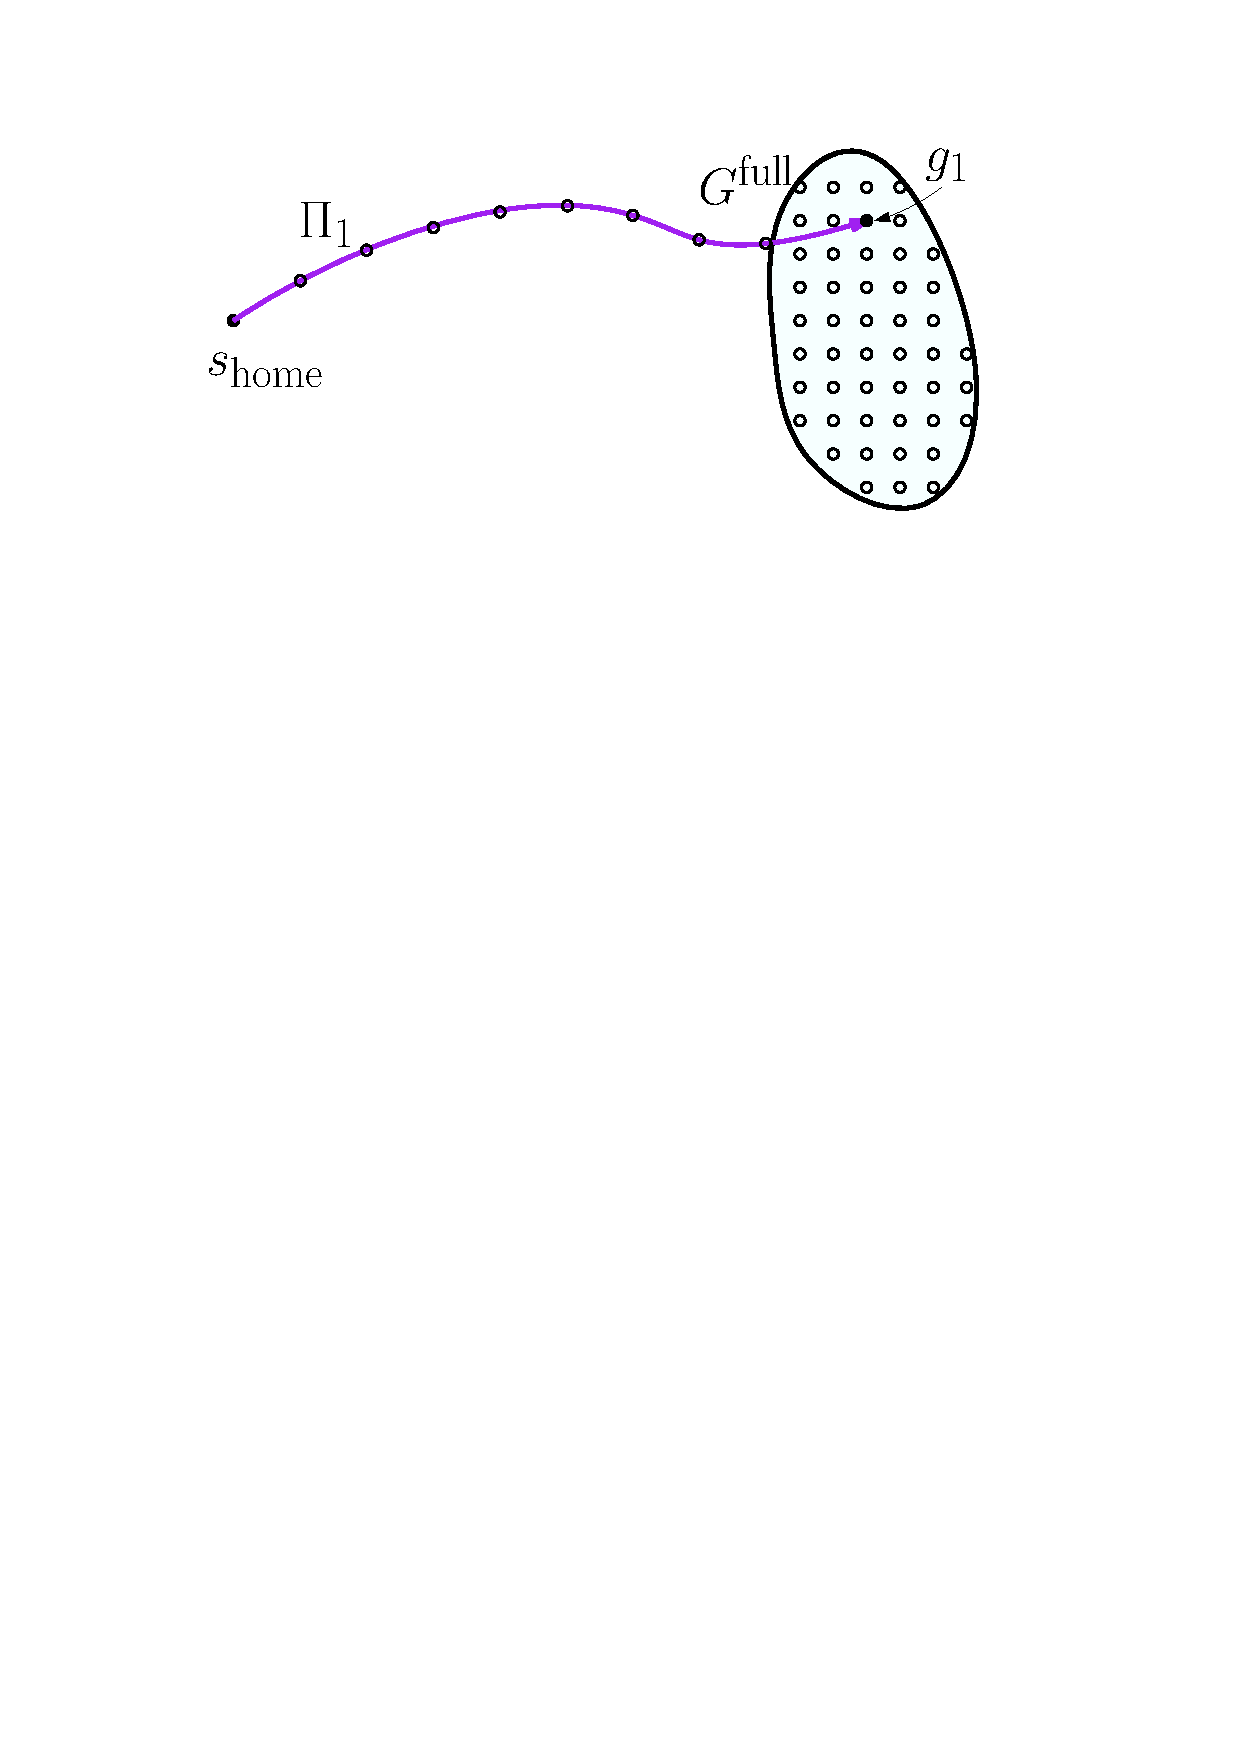
\includegraphics[width=\textwidth]{2_compute_root_paths_1}
        \caption{}
        \label{fig:crp1}
    \end{subfigure}
    \hspace{4mm}
    \begin{subfigure}{0.225\textwidth}
    %   \centering
        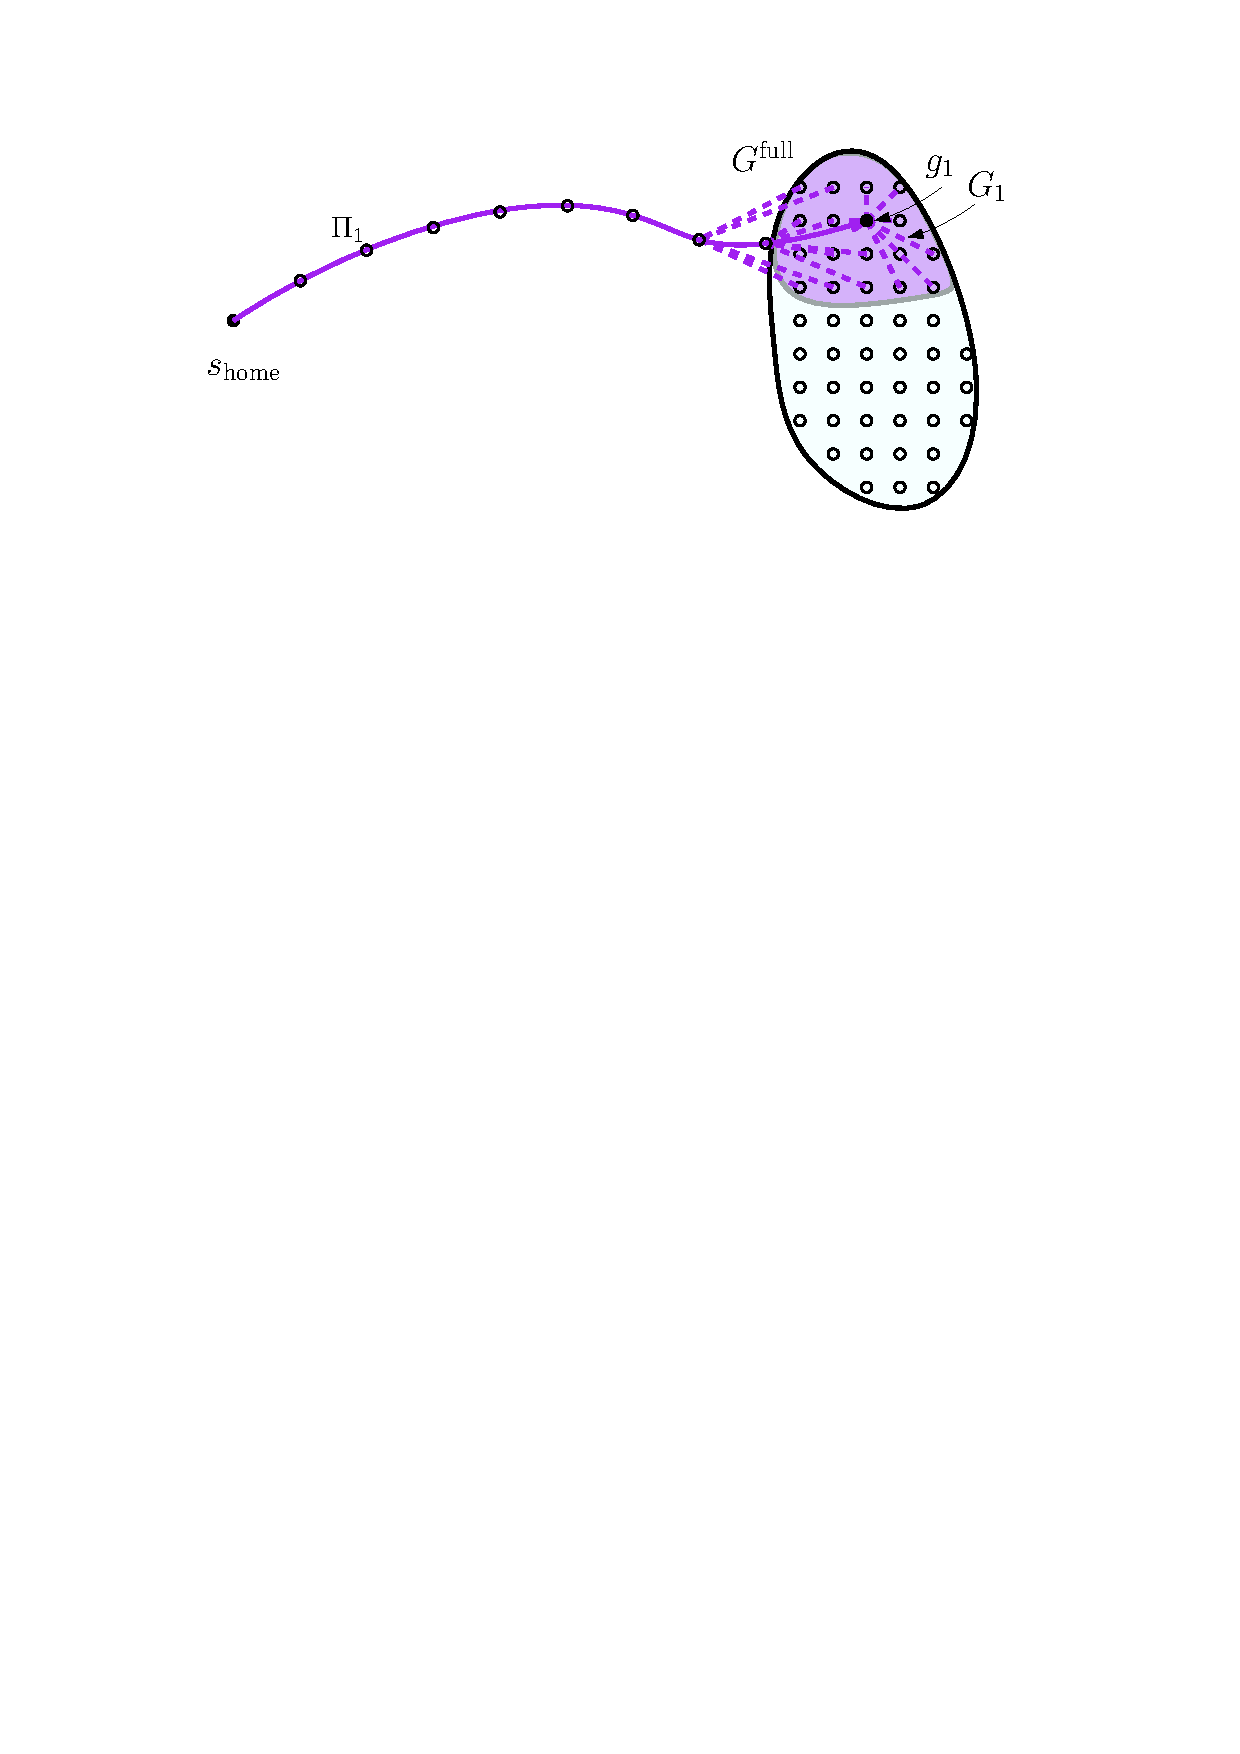
\includegraphics[width=\textwidth]{2_compute_root_paths_2}
        \caption{}
        \label{fig:crp2}
    \end{subfigure}
    \hspace{4mm}
    \begin{subfigure}{0.225\textwidth}
    %   \centering
        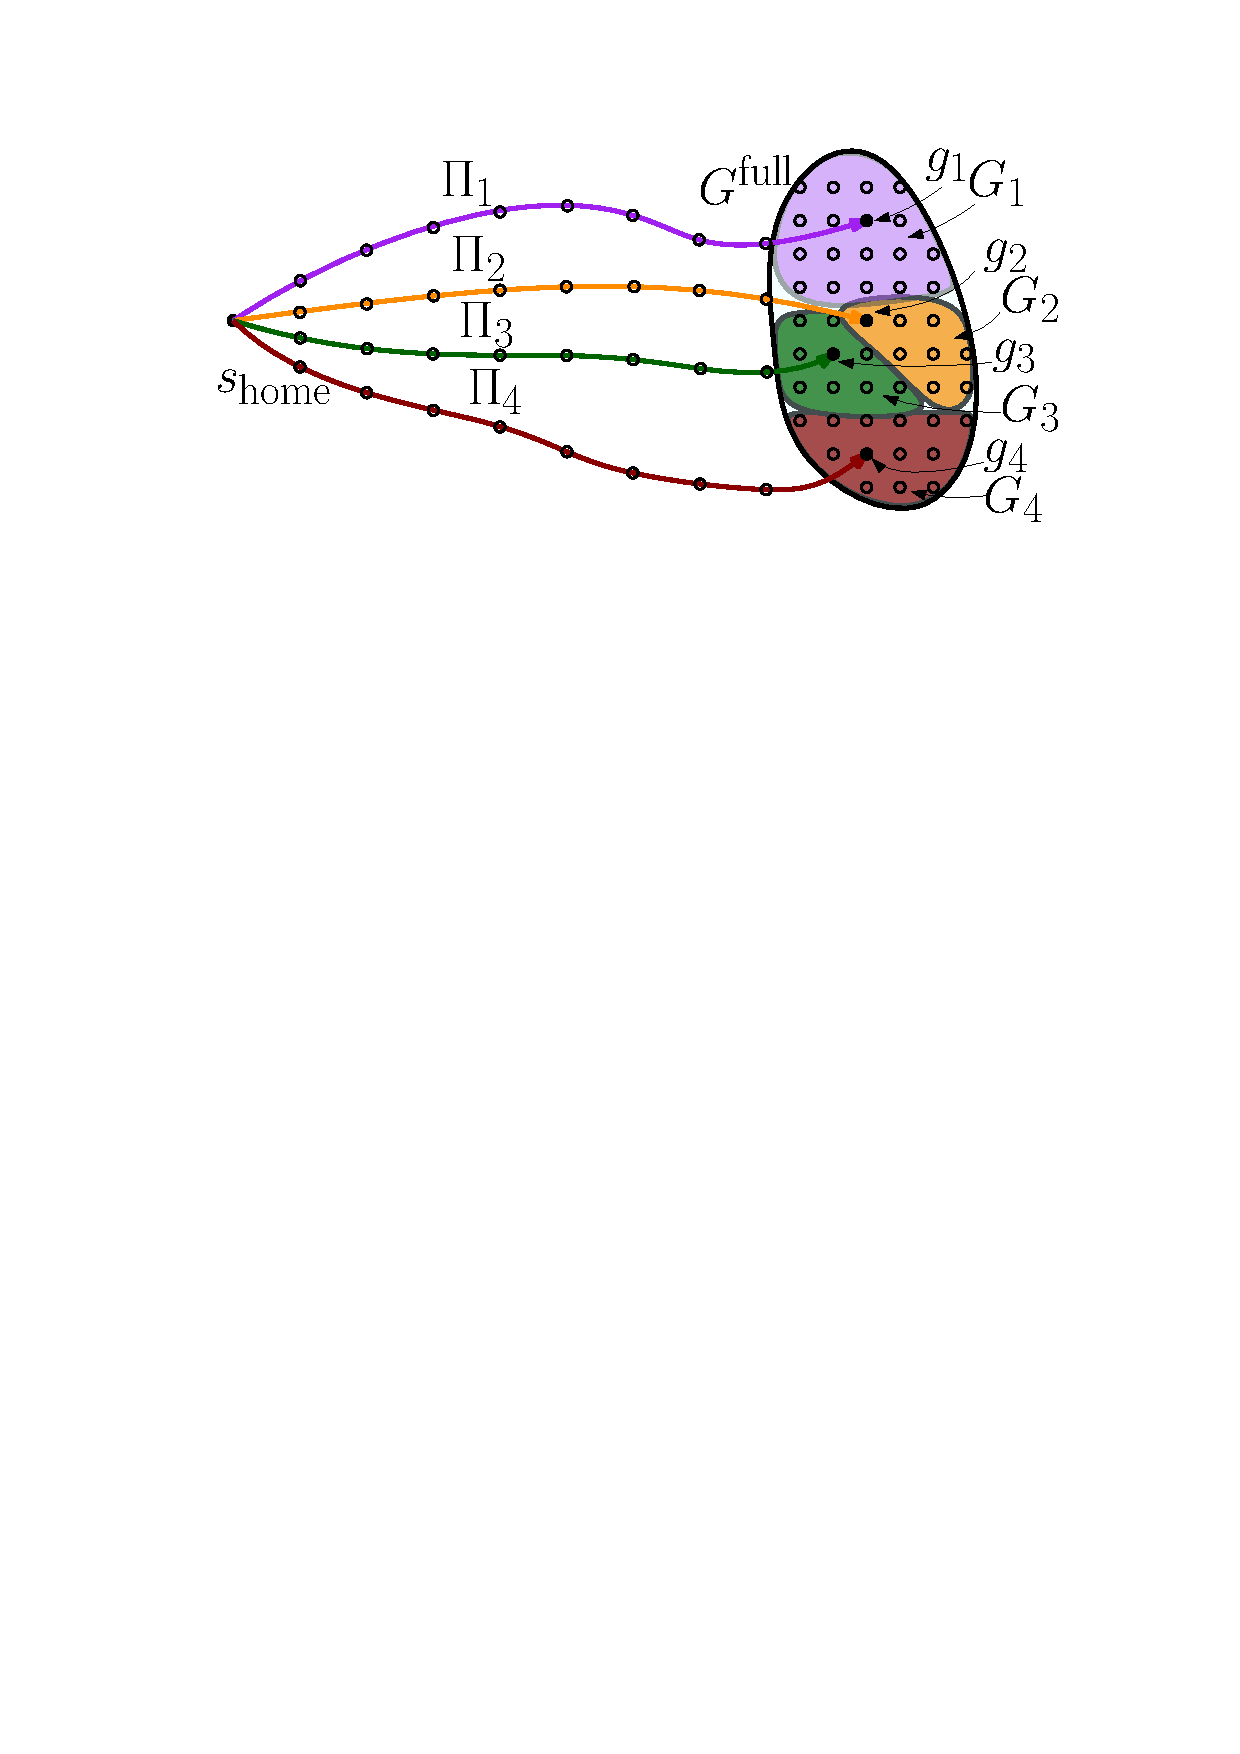
\includegraphics[width=\textwidth]{2_compute_root_paths_3}
        \caption{}
        \label{fig:crp3}
    \end{subfigure}
    \caption{\CaptionTextSize
    First step of the preprocessing stage.
    (\subref{fig:crp1})~A goal state $g_1$ is sampled and the root path $\Pi_1$ is computed between \Shome and $g_1$.
    %
    (\subref{fig:crp2})~The set $G_1 \subset \Gfull$ of all states that can use $\Pi_1$ as an experience is computed and associated with $\Pi_1$.
    %
    (\subref{fig:crp3})~The goal region covered by four root paths from \Shome after the first step of the preprocessing stage terminates.
    }
    \label{fig:crp}
    \vspace{-5mm}
\end{figure*}
Our preproccesing stage starts by sampling a goal state~$g_1 \in \Gfull$ and computing a root path~$\Pi_1$ from~$\Shome$ to~$g_1$. We then associate with~$\Pi_1$ all goal states~$G_1 \subset \Gfull$ such that~$\Pi_1$ can be used as an experience in reaching any state in $g_1' \in G_1$ within~\Tbound
Thus, all goal states in~$G_1$ are covered by~\Shome.
%
We then repeat this process but instead of sampling  a goal state from \Gfull, we sample from $\Gfull \setminus \Gcov$, where~\Gcov is the set of goal states already covered by \Shome.
At the end of this step, we obtain a set of root paths. 
Each root path~$\Pi_i$ is associated with a goal set $G_i \subseteq \Gfull$ such that 
(i)~$\Pi_i$ can be used as an experience in reaching any state in $g_i' \in G_i$ in~\Tbound and 
(ii)~$\bigcup_i G_i = \Gfull$.
%
See Fig.~\ref{fig:crp}.and  Alg.~\ref{alg:step1}, respectively.




\begin{algorithm}[t]
\caption{\textsc{ComputeRootPaths}($s_{\textrm{start}}, \Guncov$)}
\label{alg:step1}
    \AlgFontSize
\begin{algorithmic}[1]
\State $\Psi \leftarrow \emptyset$   \Comment{A list of pairs ($\Pi_i, G_i)$}
\State $\Guncovp \leftarrow \emptyset$; \hspace{3mm}
       $\Gcovp \leftarrow \emptyset$; \hspace{3mm}
       $i = 0$
\While{$\Guncov \neq \emptyset$}
        \Comment{Runs until all uncovered points are considered}
    \State $g_i \leftarrow$\textsc{Sample}($\Guncov$)
    \State $\Guncov \leftarrow \Gcov \setminus \{g_i\}$
    
    \State $\Pi_i \leftarrow$ \textsc{Plan}($s_{\textrm{start}}, g_i$)
        \Comment{Plans root path}
    \If {$\Pi_i = \emptyset$}  \Comment{Path does not exist}
        \State $\Guncovp \leftarrow \Guncovp \cup \{g_i\}$
    \Else
        \State $G_i \leftarrow \{ g_i \}$
        \For {\textbf{each} $g_j \in \Guncov$}
            \State $\pi_j \leftarrow$\textsc{Plan}($s_{\textrm{start}},g_j,\Pi_i$)
                \Comment{Plans using root path as experience}
            \If {$\pi_j \neq \emptyset$} \Comment{Planner succeeded}
                \State $G_i \leftarrow G_i \cup \{g_j\}$
                \State $\Guncov \leftarrow \Guncov \setminus \{g_j\}$
            \EndIf
        \EndFor
        \State $\Psi \leftarrow \Psi \cup \{ (\Pi_i, G_i)\}$
        \Comment{Insert $(\Pi_i, G_i)$ to $\Psi$}
        \State $i \leftarrow i + 1$
    \EndIf
\EndWhile
\State \textbf{return} $\Psi, \Guncovp$
\end{algorithmic}
\end{algorithm}



%%%%%%%%%%%%%%%%%%%%%%%%%%%%%%%%%%%%%%%%%%%%%%%%%%%%
\begin{algorithm}[t]
\caption{\textsc{PreprocessMain(\Shome, \Gfull)}}\label{alg:all}
    \AlgFontSize
\begin{algorithmic}[1]
    \State \textsc{Preprocess}($\Shome, \Gfull$)
\end{algorithmic}
\end{algorithm}
%
\begin{algorithm}[t]
\caption{\textsc{Preprocess}($\Sstart,\Guncov,\Gcov $)}\label{alg:preprocess}
    \AlgFontSize
\begin{algorithmic}[1]
\State $\Psi_{\textrm{work}}, G'^{\textrm{uncov}}_{\textrm{work}} \leftarrow$ \textsc{ComputeRootPaths}($\Sstart,\Guncov$)

\If {$\Sstart = \Shome$}
    \State $\Psi_{\textrm{home}} = \Psi_{\textrm{work}}$
\EndIf

\State $G'^{\textrm{cov}} \leftarrow 
    \Gcov \cup (\Guncov \setminus G'^{\textrm{uncov}}_{\textrm{work}})$
\If{$t(s_{\textrm{start}}) \geq \Trc$}
    \State \textbf{return} $G'^{\textrm{uncov}}_{\textrm{work}}, G'^{\textrm{cov}}$
\EndIf
\For {\textbf{each} $(\Pi_i, G_i) \in \Psi_{\textrm{work}}$}
    \State $G_i^{\textrm{cov}} \leftarrow G_i$;
            \hspace{2mm}
           $G_i^{\textrm{uncov}} \leftarrow G'^{\textrm{cov}} \setminus G_i$;
            \hspace{2mm}
           $t = \Trc$
%    \State $t = \Trc$
%    \State $G_i^{\textrm{UNCOV}} \leftarrow G'^{\textrm{COV}} \setminus G_i$
%    \State $G_i^{\textrm{COV}} \leftarrow G_i$

    \While{$t \geq t(\Sstart)$}
        \State $s \leftarrow$ \textsc{GetState($\Pi_i, t$)}
        \For {\textbf{each} $(\Pi_j, G_j) \in \Psi_{\textrm{home}}$}
        \label{alg:preprocess:line:latch1a}
            \If{\textsc{CanLatch}($s,\Pi_j$)}
                \State $G_i^{\textrm{uncov}} \leftarrow G_i^{\textrm{uncov}} \setminus G_j$
                \State $G_i^{\textrm{cov}} \leftarrow G_i^{\textrm{cov}} \cup G_j$
                \label{alg:preprocess:line:latch1b}
            \EndIf
        \EndFor
        % }
        %%%%%%%%% LATCHING END
        \If{$G_i^{\textrm{uncov}} = \emptyset$}
            \State \textbf{break}
        \EndIf
        \State $G_i^{\textrm{uncov}},G_i^{\textrm{cov}} \leftarrow$ \textsc{Preprocess}($s,G_i^{\textrm{uncov}},G_i^{\textrm{cov}}$)
        \If{$G_i^{\textrm{uncov}} = \emptyset$}
            \State \textbf{break}
        \EndIf
        \State $t \leftarrow t - \delta_t$
    \EndWhile
    % \State $(\Pi_i,\Pi_j).s = s$ \Comment{replan state}
\EndFor
\State \textbf{return} $G'^{\textrm{uncov}}_{\textrm{work}}, G'^{\textrm{cov}}$

\end{algorithmic}
\end{algorithm}

%%%%%%%%%%%%%%%%%%%%%%%%%%%%%%%%%%%%%%%%%%%%%%%%%%%%

Equipped with a set of root paths and the corresponding goal regions they cover, we now need to allow for efficient replanning. This is done by using the following two observations:
\begin{enumerate}[label={\textbf{O\arabic*}},leftmargin=0.75cm]
    \item \label{obs:1} 
    Assume that $\calR$ is executing a path $\Pi_i$ to $g_i \in G_i$ and that $\Pi_{s, i \rightarrow j}$ is a path starting at state $s \in \Pi_i$ and ending at goal $g_j \in \Gfull \setminus G_i$.
    If the last update given by $\calP$ happens $\Tbound + \delta_t$ before $s$ is reached,
    then the system can execute path $\Pi_i$ until $s$ and then continue executing $\Pi_{s, i \rightarrow j}$ to reach  $g_j$.

    \item \label{obs:2} 
    Assume that $\calR$ is executing a path $\Pi_i$ to $g_i \in G_i$ and that $\pi_{s,s',i \rightarrow j}$ is a path connecting  $s \in \Pi_i$ to $s' \in \Pi_j$ (with~$\Pi_j$ the root path to $g_j \in G_j$).
    If the last update given by~$\calP$ happens $\Tbound + \delta_t$ before~$s$ is reached,
    and the new goal is in $G_j$,
    then the system can execute path~$\Pi_i$ until~$s$, execute $\pi_{s,s',i \rightarrow j}$ and then continue executing~$\Pi_{j}$ from~$s'$ until the goal is reached.

    %\os{do we need to add a figure???}
\end{enumerate}

%\subsubsection{Procrastination is a bliss}
%Recall that in the straw man algorithm presented in Sec.~\ref{subsec:strawman}, given a path $\Pi$ connecting \Shome to some goal $g$, we computed a path to every goal state $\Gfull \setminus \{g\}$ from all replanable states.
%
\ref{obs:1} implies that if we can cover a goal state $g'$  by some state~$s$ along $\Pi_g$ (with $g \neq g'$), then we cover $g'$ by all states $\Pi$ that occur before~$s$.
%
\ref{obs:2} implies that if we can compute a path connecting one root path to some other root path, a process we term as ``latching'' on to the new path, then the new root path can be used to reach all its associated goal states.

We are now ready to describe the second step of our preprocessing stage.
%
For every root path $\Pi_i$ we look at the last replanning state $s_{\Pi_i, \Trc}$ (namely, the state that is $t=\Trc$ time from \Shome). For every other root path $\Pi_j$, we test if the motion (a dynamically generated primitive) connecting $s_{\Pi_i, \Trc}$ to $s_{\Pi_j, \Trc + \delta_t}$ (the state on $\Pi_j$ that is $\Trc+\delta_t$ away from \Shome) is valid (i.e. is collision free and reachable in time). 
%
If this is the case then all goal states in $G_j$ are covered by all replanning states along~$\Pi_i$
See Alg.~\ref{alg:preprocess} lines~\ref{alg:preprocess:line:latch1a}-\ref{alg:preprocess:line:latch1a}.
%

Let $\Guncov(\Trc)$ be all the states that are still uncovered after the above process. We recursively apply our algorithm to the setting where the start state is $s_{\Pi_i, \Trc}$ and the goal region is~$\Guncov(\Trc)$.
If all states are covered after this step, we terminate. 
If not, let $\Guncovp(\Trc)$ be all the states still uncovered.
We consider the state $s_{\Pi_i, \Trc-\delta_t}$ (the state on $\Pi_j$ that is $\Trc-\delta_t$ away from \Shome) and recursively run our algorithm where the start state is $s_{\Pi_i, \Trc-\delta_t}$ and the goal region is $\Guncovp(\Trc)$.
This process is repeated until either all states are covered or we backtracked to $s_{\Pi_i, 0}$ i.e the first state on $s_{\Pi_i}$.
See Fig.~\ref{fig:pl} and  Alg.~\ref{alg:all} and~\ref{alg:preprocess}, respectively.

Thus, the outcome of the preprocessing stage is map $\calM: S \times \Gfull \rightarrow \{ \Pi_1, \Pi_2, \ldots \}$ mapping which root path can be as an experience to reach a goal $g$ from a state $s$.






\begin{figure*}[t]
    \centering
    \begin{subfigure}{.225\textwidth}
    %   \centering
        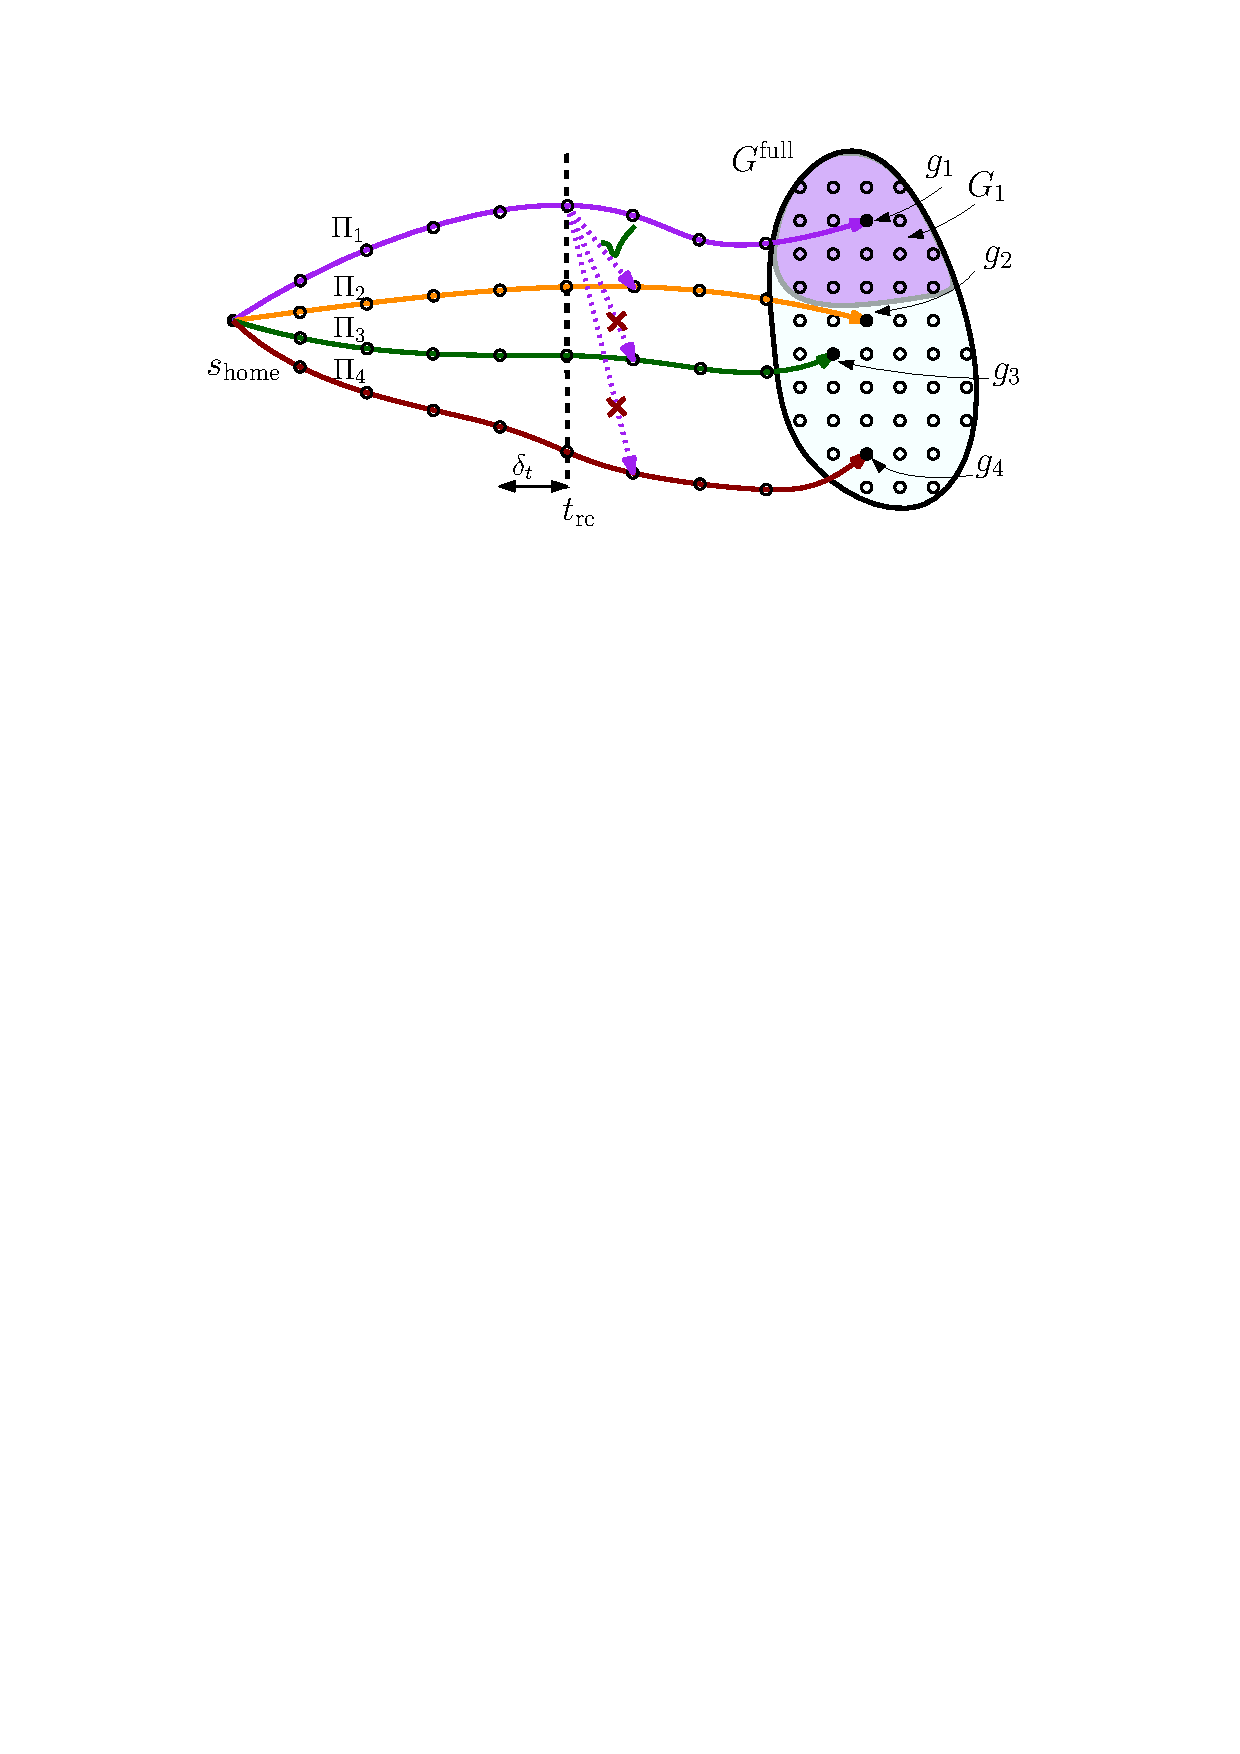
\includegraphics[width=\textwidth]{3_preprocess_loop_1}
        \caption{}
        \label{fig:pl1}
    \end{subfigure}
    \hspace{1mm}
    \begin{subfigure}{0.225\textwidth}
    %   \centering
        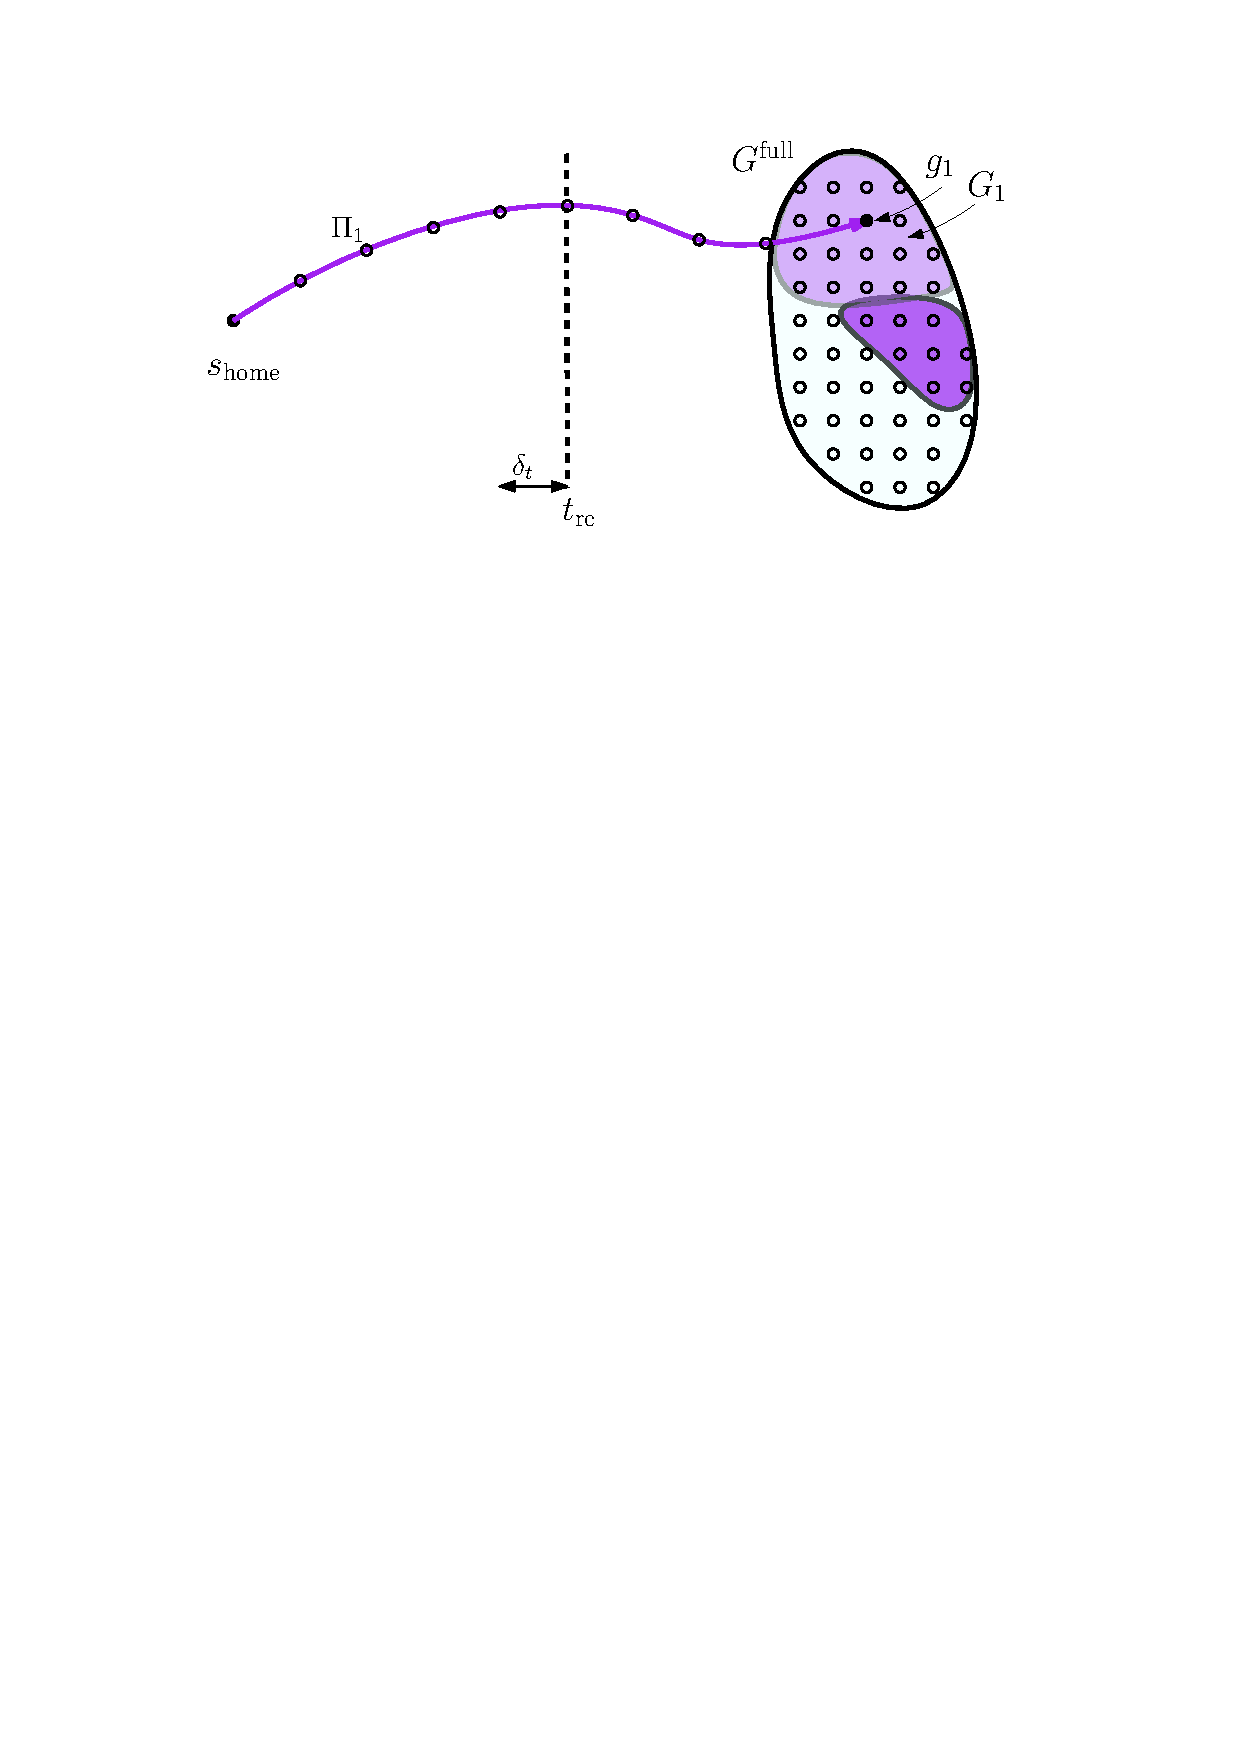
\includegraphics[width=\textwidth]{3_preprocess_loop_2}
        \caption{}
        \label{fig:pl2}
    \end{subfigure} 
    \hspace{1mm}
    \begin{subfigure}{0.225\textwidth}
    %   \centering
        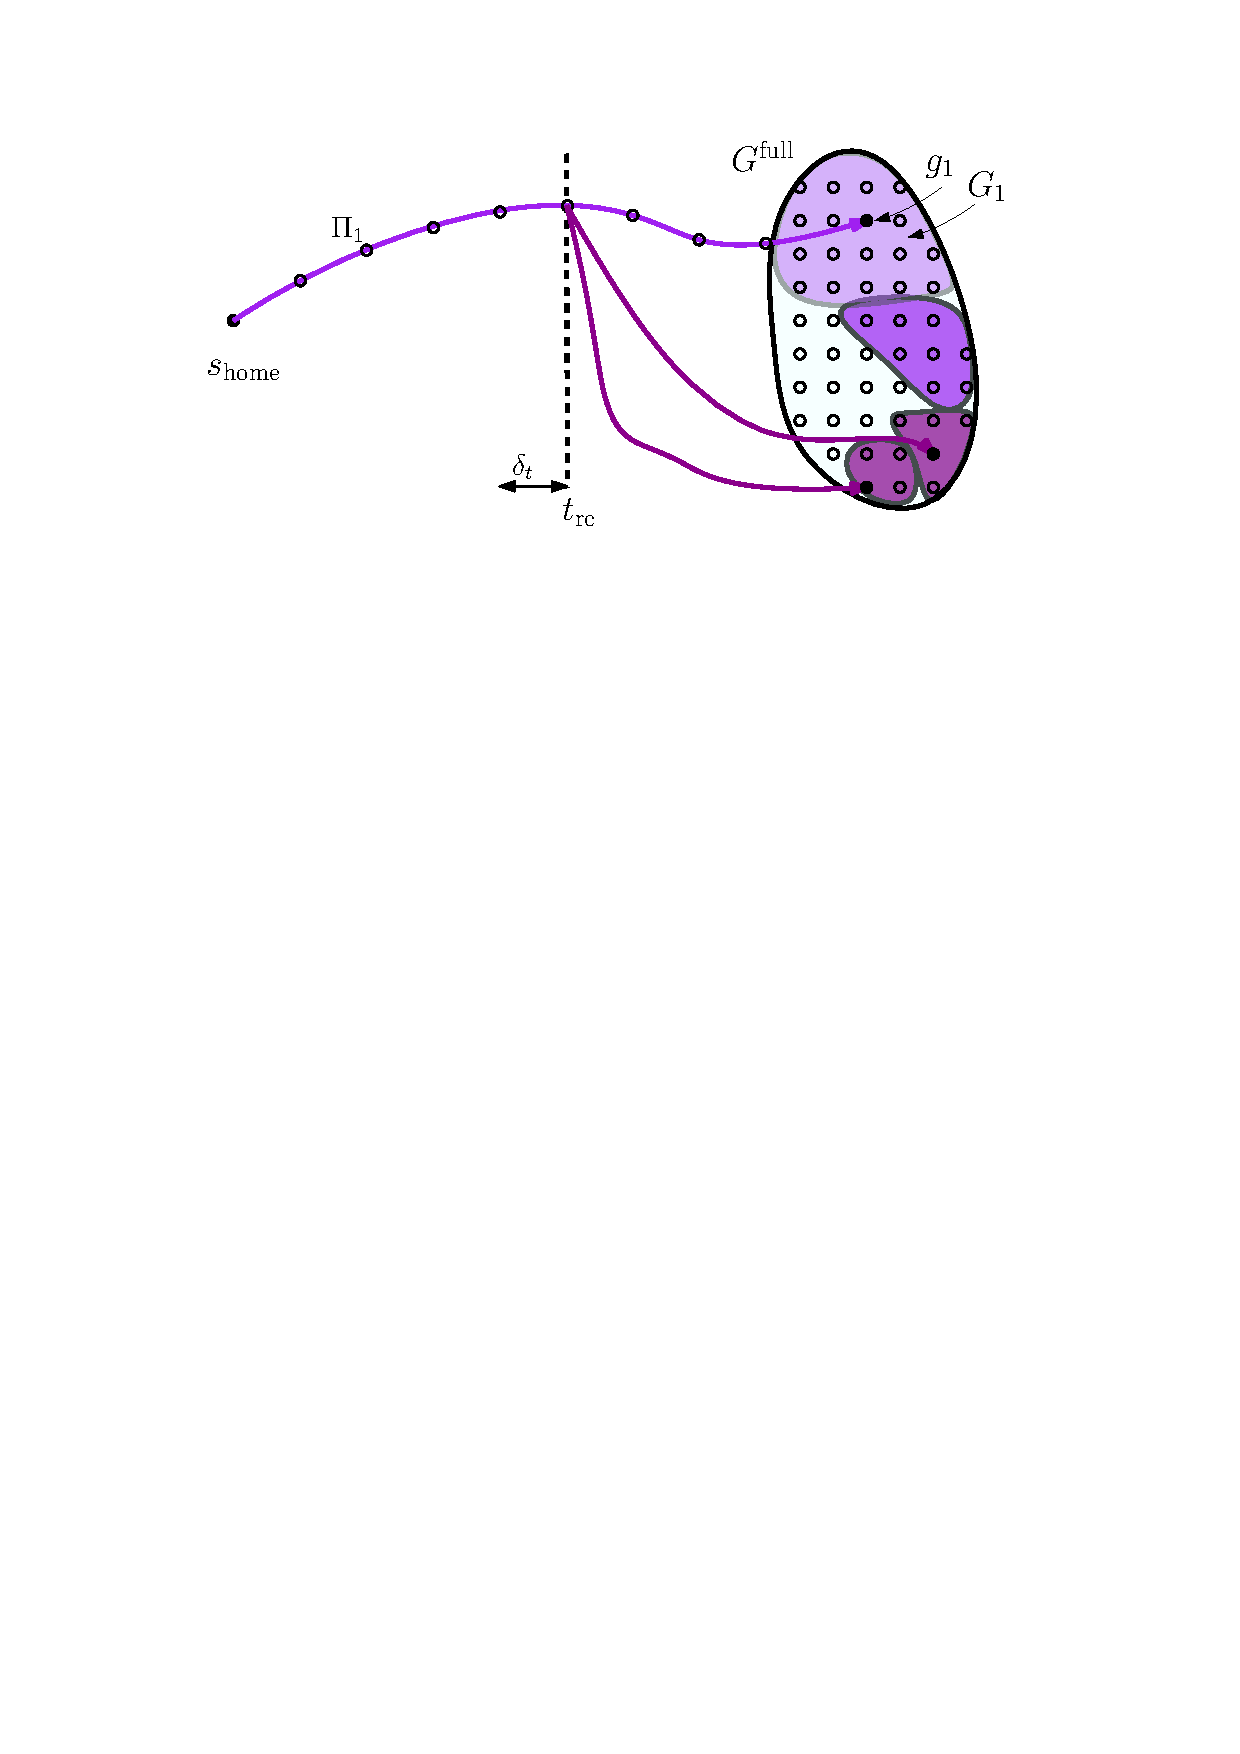
\includegraphics[width=\textwidth]{3_preprocess_loop_3}
        \caption{}
        \label{fig:pl3}
    \end{subfigure}
    %
    \hspace{1mm}
    \begin{subfigure}{.225\textwidth}
    %   \centering
        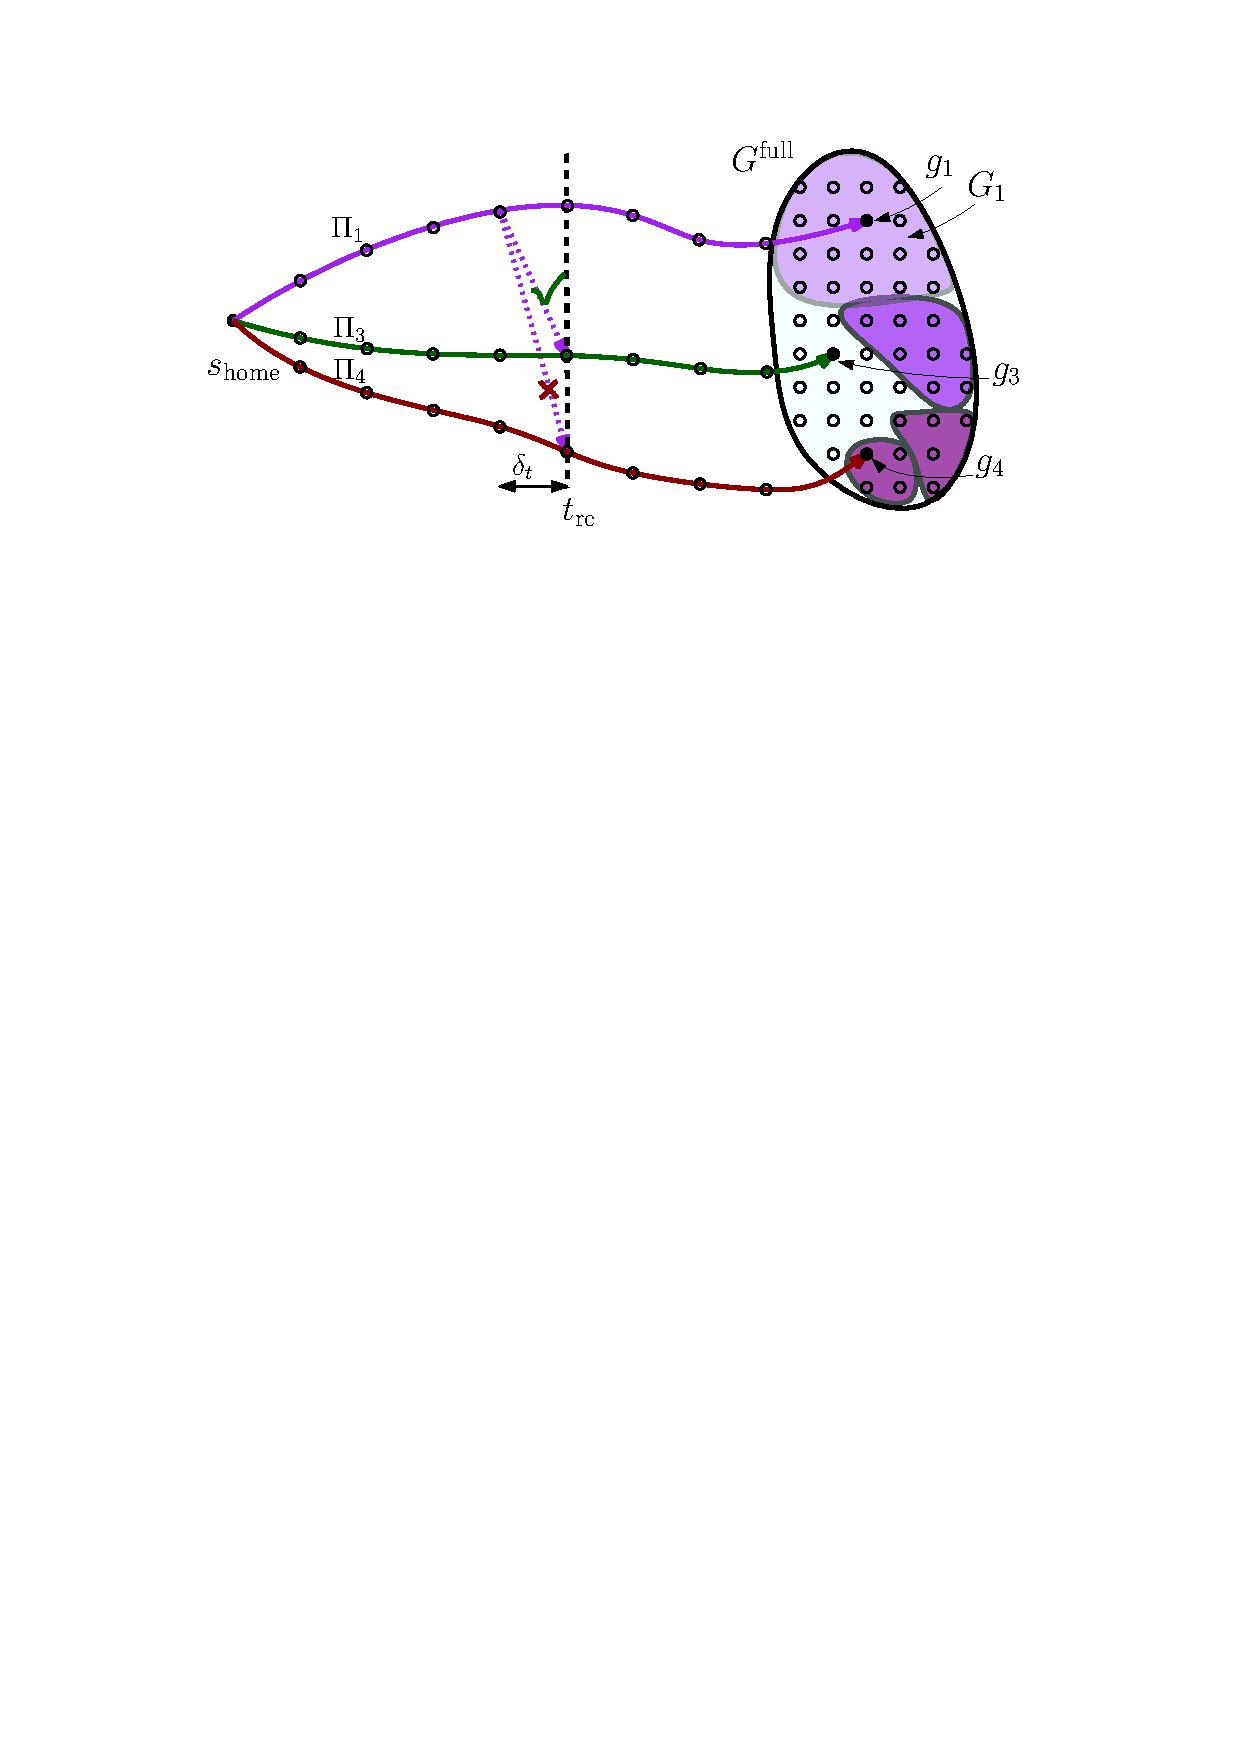
\includegraphics[width=\textwidth]{3_preprocess_loop_4}
        \caption{}
        \label{fig:pl4}
    \end{subfigure}
    %\hspace{2mm}
    \begin{subfigure}{0.225\textwidth}
    %   \centering
        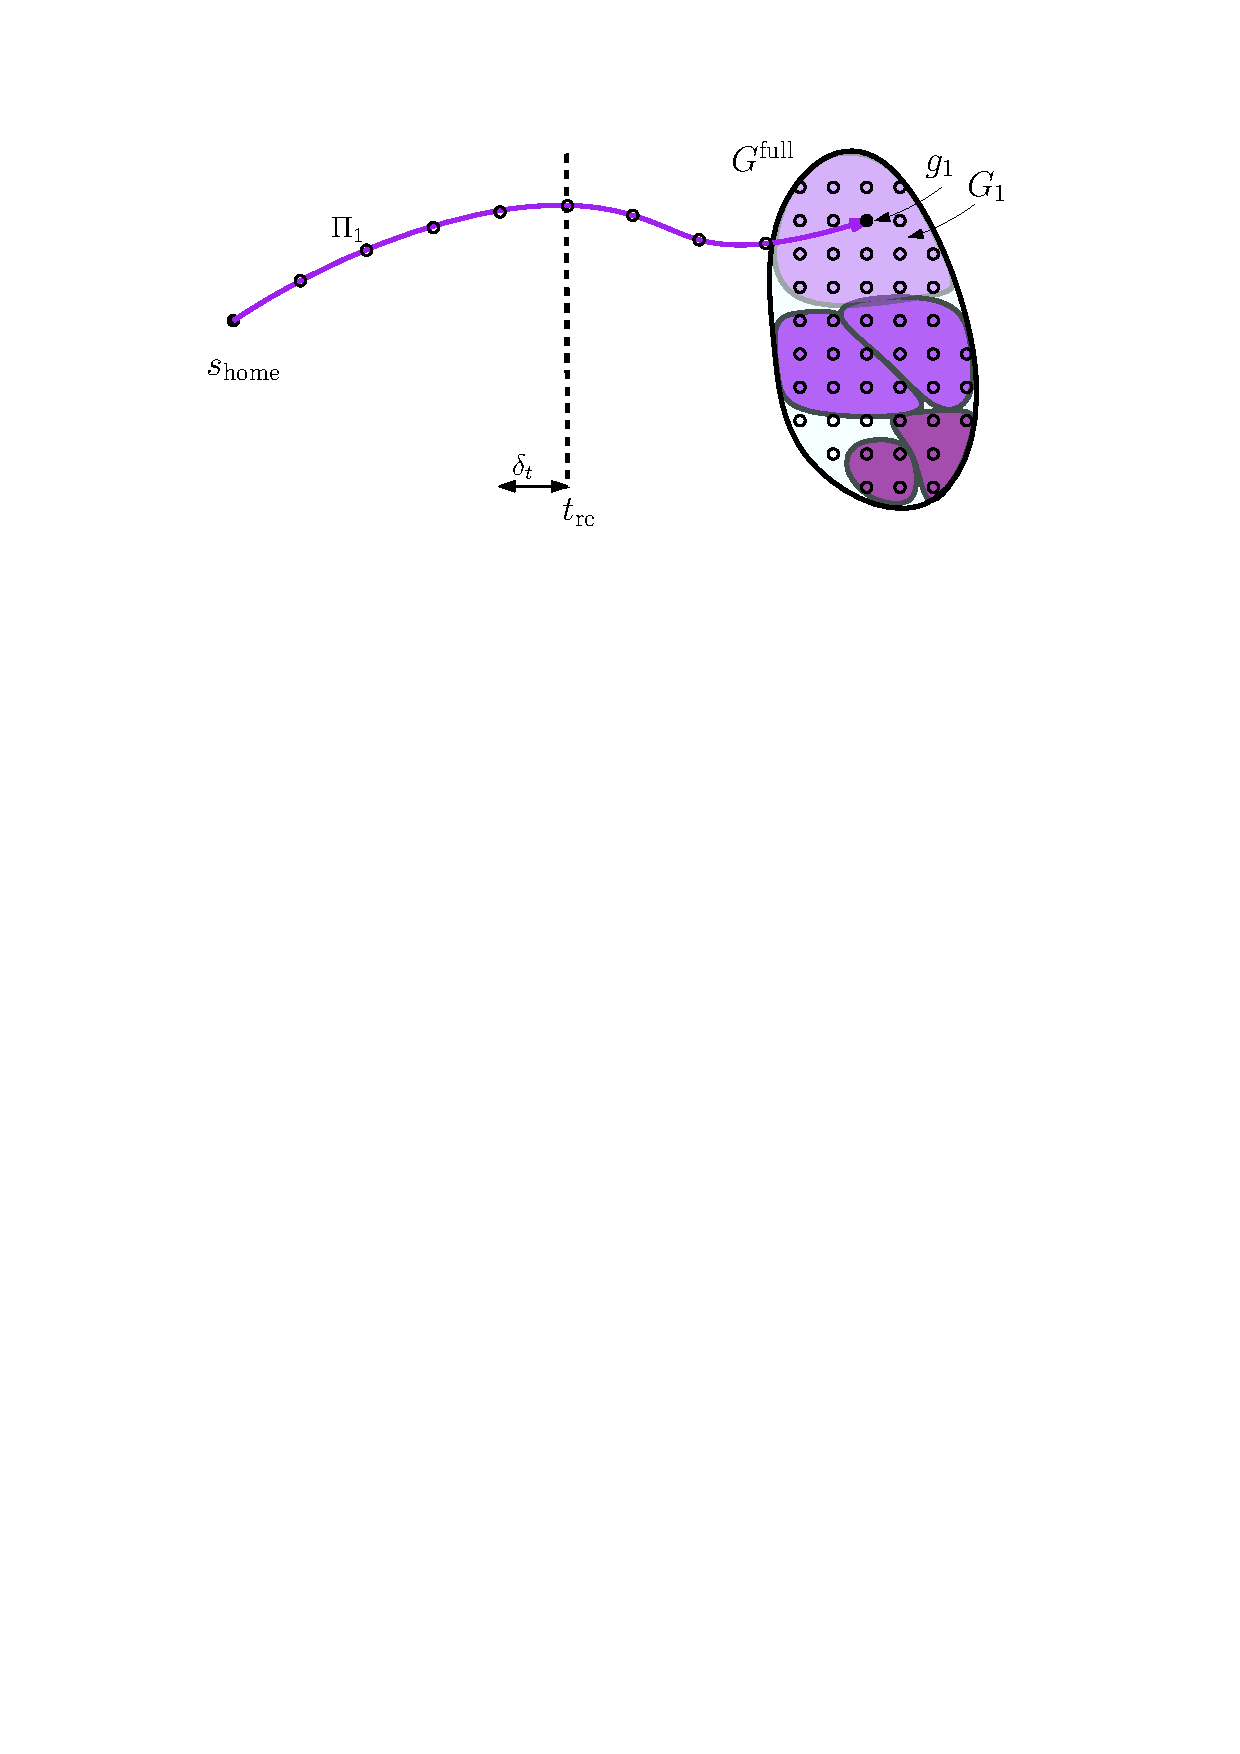
\includegraphics[width=\textwidth]{3_preprocess_loop_5}
        \caption{}
        \label{fig:pl5}
    \end{subfigure}
    \hspace{1mm}
    \begin{subfigure}{0.225\textwidth}
    %   \centering
        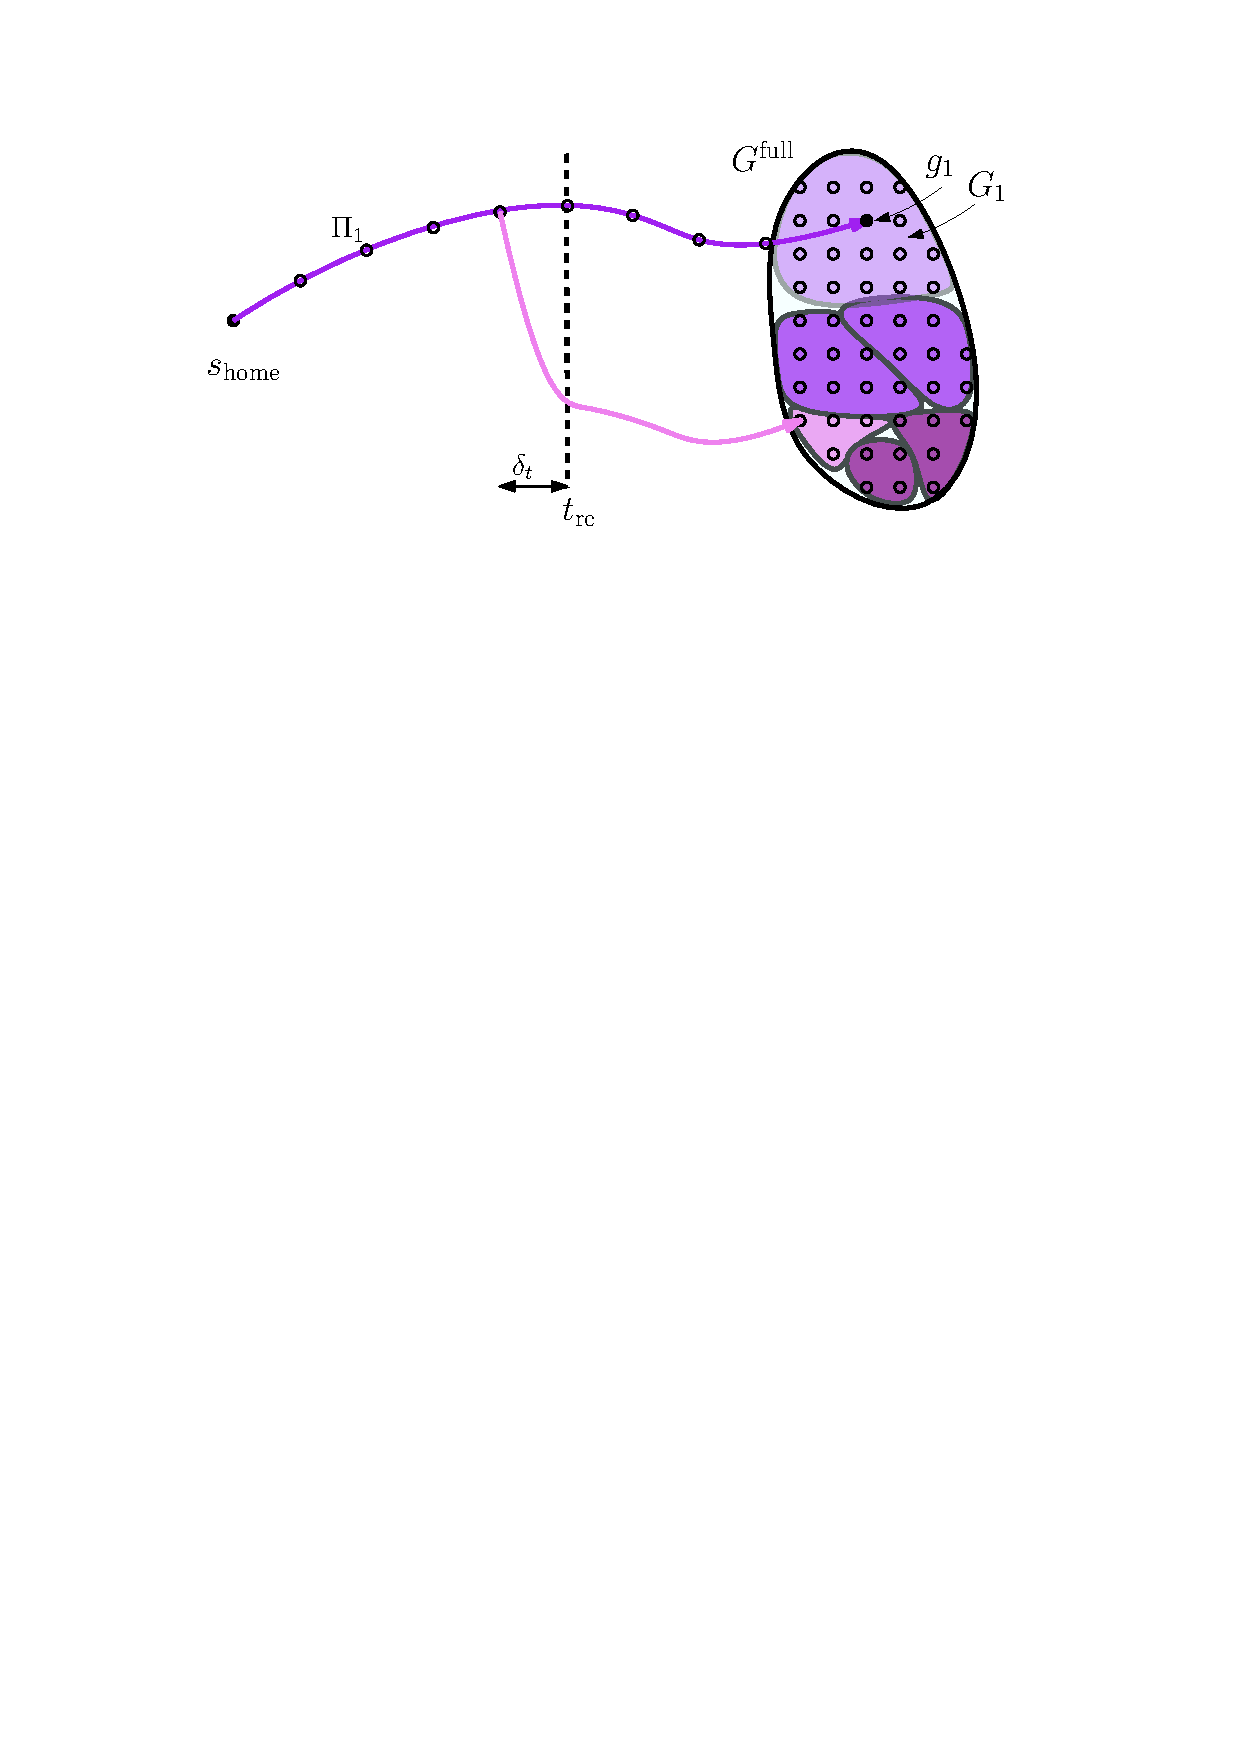
\includegraphics[width=\textwidth]{3_preprocess_loop_6}
        \caption{}
        \label{fig:pl6}
    \end{subfigure}
    \hspace{1mm}
    \begin{subfigure}{0.225\textwidth}
    %   \centering
        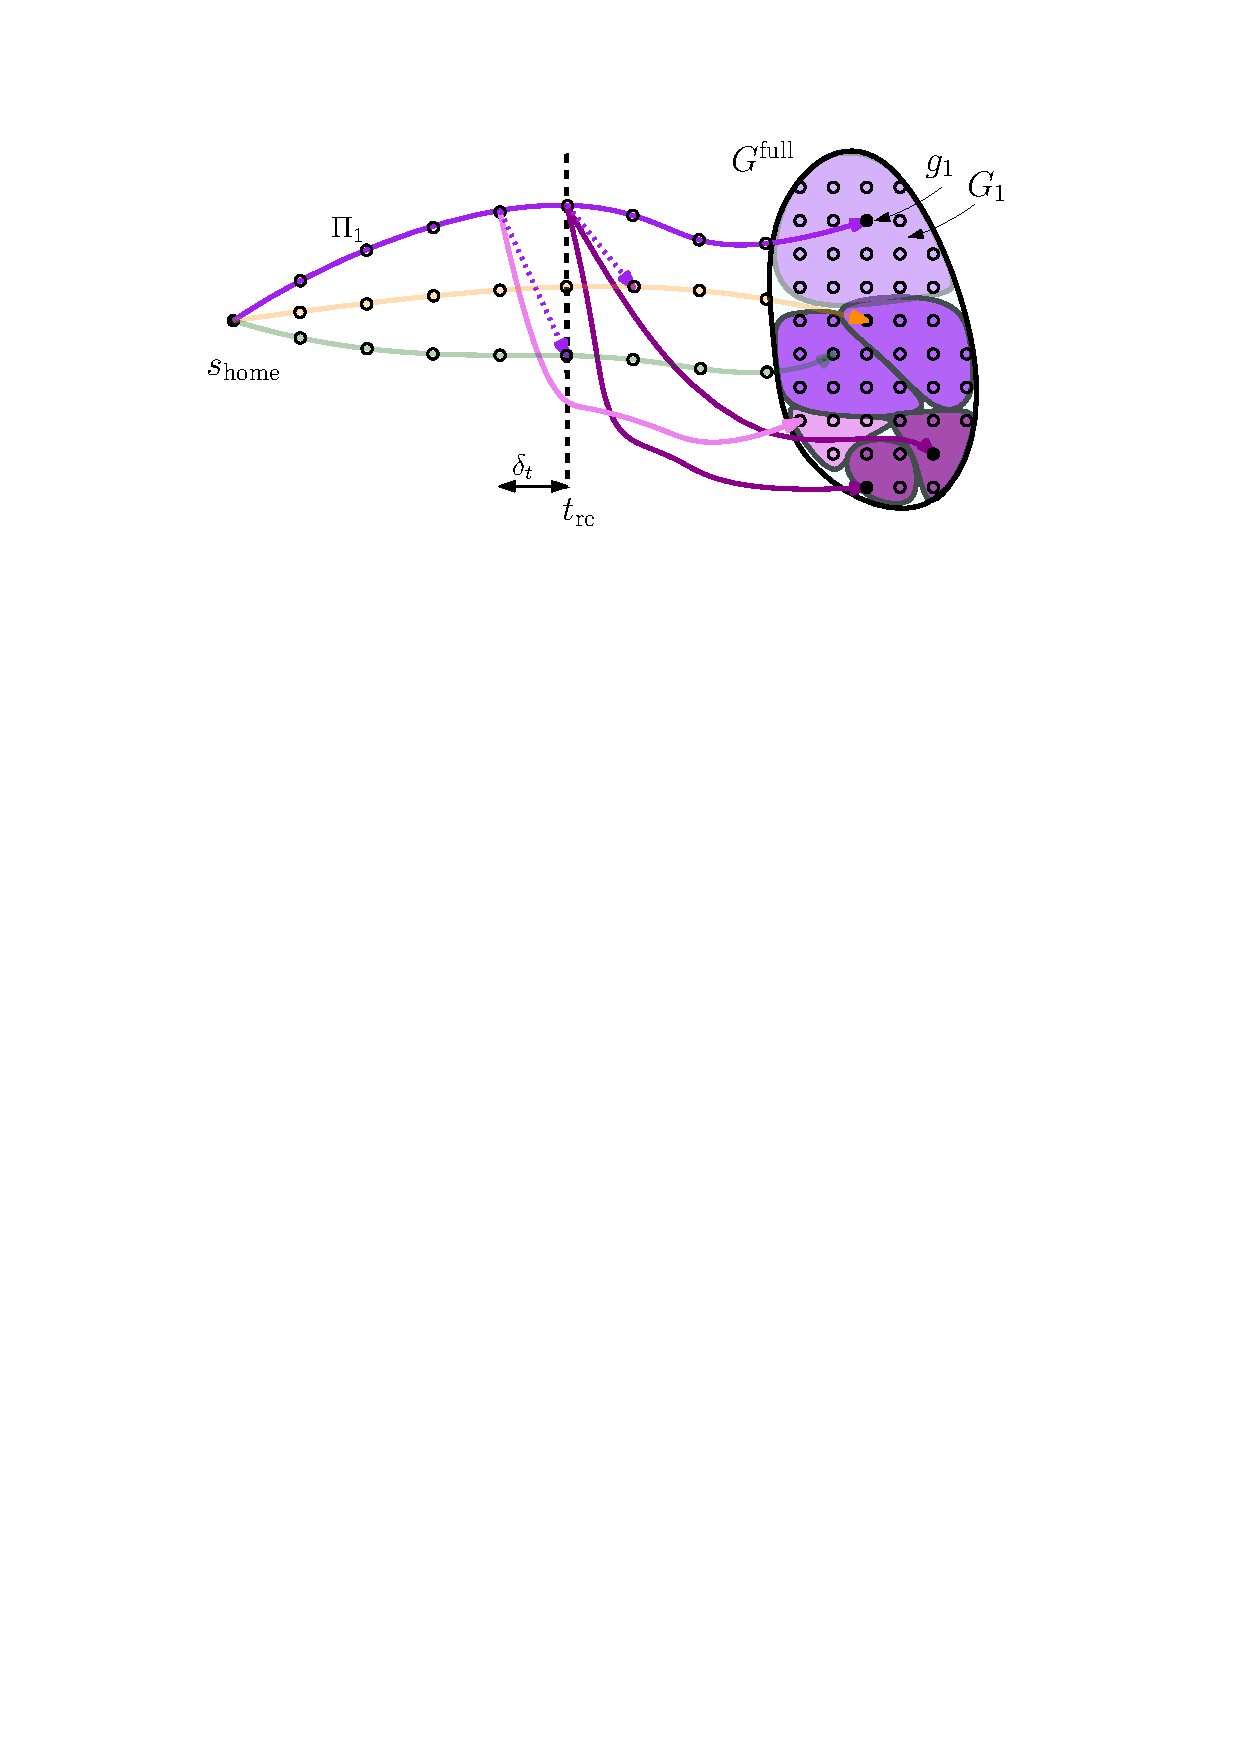
\includegraphics[width=\textwidth]{3_preprocess_loop_7}
        \caption{}
        \label{fig:pl7}
    \end{subfigure}
    \caption{\CaptionTextSize
    Preprocess loop.
    (\subref{fig:pl1})~We start by trying to latch on to every other root path. 
    %
    (\subref{fig:pl2})~For successful latches, we add the corresponding goal states to our covered region.
    %
    (\subref{fig:pl3})~We then try to compute new root path with its corresponding goal states (see also Fig.~\ref{fig:crp2}).
    %
    (\subref{fig:pl4})-(\subref{fig:pl6})~This process is repeated by backtracking along the root path.
    %
    (\subref{fig:pl7})~Outcome of a preprocessing step for one path. \Gfull is covered either by using $\Pi_1$ as an experience, 
    latching on to $\Pi_2$ or  $\Pi_3$ (at different time steps)
    or by 
    using newly-computed root paths. 
    }
    \label{fig:pl}
    \vspace{-5mm}
\end{figure*}

\subsubsection{Query}
In the query stage, given an initial estimation $g_{\rm init}$ of the goal pose from $\calP$, our algorithm queries $\calM$ to obtain the root path $\Pi$ from $\Shome$ to $g_{\rm init}$.
It then plans a path using $\Pi$ as an experience and starts executing this path.
%
Now, assume that the~$\calR$ is executing path $\Pi_{\rm curr}$ and a new estimation $g_{\rm new}$ of the goal pose is provided by $\calP$.
%
We consider the state $s_{\Pi_{\rm curr}, \Trc}$ along the path $\Pi_{\rm curr}$ at time $\Trc$ and test if
(i)~we can reuse the root path that $\calR$ is currently executing as an experience to reach the new goal
(Alg.~\ref{alg:query}, lines~\ref{alg:query:line:c1a}-\ref{alg:query:line:c1b}),
(ii)~there is a root path that can be used as an experience to reach $g_{\rm new}$ starting at $s_{\Pi_{\rm curr}, \Trc}$ 
(Alg.~\ref{alg:query}, lines~\ref{alg:query:line:c2a}-\ref{alg:query:line:c2b})
or if 
(iii)~there is a root path starting at \Shome associated with~$g_{\rm new}$ that we can latch on to.
If the former holds, we run our experience-based planner to obtain a path $\Pi(s_{\Pi_{\rm curr}}, \Trc, g_{\rm new})$ starting at $s_{\Pi_{\rm curr}}$ and ending at $g_{\rm new}$. We then execute $\Pi_{\rm curr}$ until $s_{\Pi_{\rm curr}, \Trc}$ and then continue by executing $\Pi(s_{\Pi_{\rm curr}}, \Trc, g_{\rm new})$.
%
If the latter holds, we run our experience-based planner to obtain a path $\Pi(s', \Trc + \delta_t), g_{\rm new})$ starting at $s'$, the state on the path we latched on to and ending at $g_{\rm new}$. We then execute $\Pi_{\rm curr}$ until $s_{\Pi_{\rm curr}, \Trc}$ and then continue by executing the motion that latches on to $s'$ and finally executing  $\Pi(s', \Trc + \delta_t, g_{\rm new})$.
See Alg.~\ref{alg:query}, lines~\ref{alg:query:line:c3a}-\ref{alg:query:line:c3b}.
%
If neither hold, we consider the state $s_{\Pi_{\rm curr}, \Trc-\delta_t}$ and repeat this process.
%
For pseudocode describing our approach see~\ref{alg:query}.

\begin{algorithm}[t]
\caption{\textsc{Query}($g, \pi_{\textrm{curr}},s_{\textrm{start}}$)}\label{alg:query}  
    \AlgFontSize
\begin{algorithmic}[1]
    \State $s_{\rm first} \leftarrow \textsc{Head}  \pi_{\textrm{curr}}$ 
        \Comment{First state on $ \pi_{\textrm{curr}}$}
        \label{alg:query:line:c1a}
    \State $\Pi_{\textrm{curr}} \leftarrow$ $\calM(s_{\textrm{start}},g)$ 
         \Comment{Lookup root path from $s_{\textrm{start}}$ to $g$}
    \State $\pi \leftarrow$ \textsc{Plan}($s_{\textrm{start}},g,\Pi_{\textrm{curr}}$)
        \Comment{Plan using root path as experience}
    \If{$\pi \neq  = \emptyset$}
        \State \textbf{return} $\pi$
        \label{alg:query:line:c1b}
    \EndIf
\vspace{2mm}

\State $t \leftarrow \Trc$; \hspace{3mm} $t_{\textrm{curr}}\leftarrow \textsc{CurrentTime} + \Tbound$
\While{$t \geq t_{\textrm{curr}}$}
    \State $s \leftarrow$ \textsc{GetState}($\pi_{\textrm{curr}}, t$)
        \Comment{Get state on path at time $t$}
        \label{alg:query:line:c2a}
    \State $\Pi_{\textrm{next}} \leftarrow$ $\calM(s,g)$ 
         \Comment{Lookup root path from $s$ to $g$}
    \If{$\Pi_{\textrm{next}} \neq \emptyset$}
        \State $\pi_{\textrm{next}} \leftarrow$\textsc{Plan}($s_{\textrm{start}},g,\Pi_{\textrm{next}}$)
         \Comment{Plan using root path as experience}
        \State $\pi \leftarrow$ \textsc{MergePaths}($\pi_{\textrm{curr}},\pi_{\textrm{next}},t$)
        \State \textbf{return} $\pi$
        \label{alg:query:line:c2b}
    \EndIf
%%%%%%%%%%%%%%%%LATCHING 

\vspace{2mm}

%    {\color{blue}
    \State $\Pi_{\textrm{home}} \leftarrow \calM (\Shome,g)$
     \Comment{Lookup root path from  to $g$}
     \label{alg:query:line:c3a}
    \If{$\Pi_{\textrm{home}} \neq \emptyset$}
        \If{\textsc{CanLatch}($s,\Pi_{\textrm{home}}$)}
            \State $\pi_{\textrm{home}} \leftarrow$\textsc{Plan}($s_{\textrm{start}},g,\Pi_{\textrm{home}}$)
            \Comment{Plan using root path}
            \State $\pi \leftarrow$ \textsc{MergePathsByLatching}($\pi_{\textrm{curr}},\pi_{\textrm{home}}, t$)
            \State \textbf{return} $\pi$
            \label{alg:query:line:c3b}
        \EndIf
    \EndIf
 %  }
%%%%%%%%%%%
    \State $t \leftarrow t - \delta_t$
\EndWhile
\State \textbf{return failure}
\end{algorithmic}
\end{algorithm}




\subsection{Theoretical guarantees}

\begin{lemma}[Completeness]
\label{lemma:completeness}
Let $s$ be a state that $\calR$ is at in the query phase and $g\in \Gfull$ is a goal state.
If~$g$ is reachable from a state $s'$ that is (i)~reachable from $s$ and (ii)~is \Tbound away from $s$ then the planner will compute a path to $g$.
\end{lemma}
We omit the proof due to lack of space.

\begin{lemma}[Constant-time planning]
\label{lemma:bounded_time}
Let $s$ be a replanable state and $g$ a goal state provided by $\calP$.
If~$g$ is reachable, the planner is guaranteed to provide a solution in constant time.
\end{lemma}

\begin{proof}
    We have to show that the query stage (Alg.~\ref{alg:query}) has a constant-time complexity. 
    The number of times the algorithm queries for a root path (namely, computing $\calM()$  which is a hash look-up that is a constant-time operation) is bounded by $n_{\textrm{steps}} = \Trc/\delta_t$ which is the maximum number of time steps from $t = 0$ to $\Trc$. 
    The number of times the algorithm will attempt to latch on to a root path (namely, a call to \textsc{CanLatch}  which is a constant-time operation) is also bounded by $n_{\textrm{steps}}$. Finally, Alg.~\ref{alg:query} calls the \textsc{Plan} method only once.
    Since we are using a deterministic planner, the computation time is constant. 
    Hence the overall complexity of Alg.~\ref{alg:query} is $O(1)$.
\end{proof}

The analysis provided in Lemma~\ref{lemma:bounded_time} highlights the tradeoff our algorithm takes.
If we use a fine discretization of states along the path (namely, we choose a small value for $\delta_t$) then the guaranteed  planning time \Tbound is going to be high but there is a higher chance that any goal $g$ will be reachable.
On the other hand, if we use a course discretization (namely, we choose a large value for $\delta_t$) then we reduce~\Tbound at the price that some goal states may not be reachable.
%




\ignore{
Before describing how this is done, consider two root paths $\Pi_i$ and $\Pi_j$ with associated goal regions $G_i$ and~$G_j$, respectively.
Now, let $s_i$ and $s_j$ be states on $\Pi_i$ and $\Pi_j$, respectively, such that the timestamp associated with $s_j$ is $\delta_t$ time after the one associated with $s_i$. Furthermore, assume that the path between $s_i$ and $s_j$ is collision free. 
%
Now, assume that the robot is executing path $\Pi_i$ (targeting a goal state in $G_i$) and the perception system updates the goal state to be reached as $g_j \in G_j$. 
If the robot did not yet reach $s_i$ then it can reach $g_j$ by
(i)~continuing to follow $\Pi_i$ until $s_i$ is reached, 
(ii)~move to $s_j$ on $\Pi_j$ and 
(iii)~use $\Pi_j$ to reach $g_j$.
%
We term the process we just described of moving from one root path to another as ``latching'' on to a new root path.

Let $s_{\Pi_i, t}$ be the state that is $t$ time from \Shome on path $\Pi_i$.
If a collision-free path existed from $s_{\Pi_i, \Trc}$ to $s_{\Pi_j, \Trc+\delta_t}$ for every $i,j$ then we could latch on from any root path to any other root path. Moreover, following Assumption~\ref{assum:4}, $\Trc$ is the last time that the perception could update the goal location so no other replanning would be required.
%
Unfortunately, this may not be the case.
%
Thus, for every root path $\Pi_i$, we consider $s_{\Pi_i, \Trc}$ and check if we can latch on to all other root paths. 
If this can't be done, then we can tr

considering the last replanning state $s_{\Pi_i, \Trc}$ (namely, the state that is $t=\Trc$ time from \Shome). For every other root path $\Pi_j$, we test if the path connecting $s_{\Pi_i, \Trc}$ to $s_{\Pi_j, \Trc + \delta_t}$ (the state on $\Pi_j$ that is $\Trc+\delta_t$ away from \Shome) is collision free. 

In the straw man algorithm this was obtained by recursively computing a path for the replanning states along all the previously-computed paths.
%
Here, we attempt to re-use the previously-computed paths as much as possible by ``latching'' onto them.




More formally, for each root path~$\Pi_i$, we start by considering the last replanning state $s_{\Pi_i, \Trc}$ (namely, the state that is $t=\Trc$ time from \Shome). For every other root path $\Pi_j$, we test if the path connecting $s_{\Pi_i, \Trc}$ to $s_{\Pi_j, \Trc + \delta_t}$ (the state on $\Pi_j$ that is $\Trc+\delta_t$ away from \Shome) is collision free. 
If this is the case we know that any goal state in $G_j$ can be
}


\section{Evaluation}
\label{sec:eval}

We evaluated our algorithm in simulation and on a real robot. The conveyor speed that we used for all of our results is $0.2m/s$. We used Willow Garage's PR2 robot in our experiments using its 7-DOF arm. The additional time dimension makes the planning problem eight dimensional.


\begin{table*}[t]
\centering
\begin{tabular}{|c||c||c|c|c||c|c|c||c|c|c|}
\hline
   & \textbf{Our Method} 
   & \multicolumn{3}{c|}{\wastar}
   & \multicolumn{3}{c|}{\textsf{E-Graph}}
   & \multicolumn{3}{c|}{\rrt}
   \\ \hline
   & $T_{b}$ = 0.2 
   & $T_{b}$ = 0.5 & $T_{b}$ = 1.0 & $T_{b}$ = 2.0 
   & $T_{b}$ = 0.5 & $T_{b}$ = 1.0 & $T_{b}$ = 2.0 
   & $T_{b}$ = 0.5 & $T_{b}$ = 1.0 & $T_{b}$ = 2.0 
   \\ \hline
Pickup success rate [\%]                   
& 92.0 & 0.0 & 0.0 & 18.0 & 0.0 & 0.0 & 80.0 & 0.0 & 0.0 & 18.0 \\ \hline
Planning success rate [\%]                  
& 94.7 & 4.0 & 17.0 & 19.0 & 31.0 & 80.0 & 90.0 & 12.0 & 9.0 & 13.0 \\ \hline
Planning time [s]
& 0.069 & 0.433 & 0.628 & 0.824 & 0.283 & 0.419 & 0.311 & 0.279 & 0.252& 0.197\\ \hline
Planning episodes per pickup 
& 3 & 2 & 2 & 2 & 2 & 2 & 2 & 2 & 2 & 2 \\ \hline
Path cost [s]                         & 10.11        & 8.19          & 8.28          & 7.60          & 8.54          & 8.22          & 7.90          & 9.68          & 8.96          & 8.04          \\ \hline
%Expansions                        & 17.57        & 315.50        & 392.81        & 495.78        & 188.24        & 202.63        & 137.02        & 146.54        & 104.75        & 78.64         \\ \hline
\end{tabular}
\caption{\CaptionTextSize Simulation results. Here $T_b$ denotes the (possibly arbitrary) timebound that the algorithm uses. Note that for our method $T_b = \Tbound$ is the time bound that the algorithm is ensured to compute a plan.}
\label{tab:sim_results}
\end{table*}



\subsection{Experimental setup}
\subsubsection{Perception system~$\calP$}
In order to pick a known object $o$ moving object along the conveyor~$\calB$, we need a method to estimate its 3-DoF pose at various locations across~$\calB$. Thus, we created an ICP-based pose estimation strategy that uses the known 3D model of~$o$ and the initial pose estimate obtained after pre-processing the input point cloud. 
%
The following process is performed at every frame obtained by $\calP$. 
We start by removing all points that lie outside $\calB$ which yields only points corresponding to the object of interest. 
This is followed by statistical outlier removal in order to remove any points that have been left in scene after the first step. 
In the final step, we compute the mean of the points left and use that as an initial translation estimate for ICP. 
The rotation estimate is applied in a way that it places the object parallel to its direction of motion along the conveyor. The object's 3D model is transformed with this initial estimate, creating a point cloud and ICP refinement is performed between this point and the pre-processed observed point cloud. The resulting transform is concatenated with the initial estimate to return the final predicted pose. For speeding up ICP, we downsample all point clouds to a leaf size of 15mm.

\subsubsection{Sense-plan-act cycle}
We follow the classical sense-plan-act cycle as depicted in Fig.~\ref{fig:tl}.
%
Specifically, 
$\calP$ captures an image (point cloud) of the object~$o$ at time~$t_{\textrm{img}}$
followed by a period of duration $T_{\textrm{perception}}$ in which the $\calP$ estimates the pose of $o$.
At time $t_{\textrm{msg}} = t_{\textrm{img}} + T_{\textrm{perception}}$, planning starts for a period of $T_{\textrm{planning}}$ which is guaranteed to be less than~$\Tbound$.
Thus, at $t_{\textrm{plan}} = t_{\textrm{msg}} + T_{\rm planning}$ the planner waits for an additional duration of $T_{\rm wait} = \Tbound - T_{\rm planning}$.
Finally, at~$t_{\textrm{exec}} = t_{\textrm{plan}} + T_{\rm wait}$, the robot starts executing the plan. Note that the goal $g$ that the planner plans for is not for the object pose at $t_{\textrm{img}}$ but its forward projection in time to $t_{\textrm{exec}}$ to account for $T_{\textrm{perception}}$ and $T_{\textrm{bound}}$.
While executing the plan, if we obtain an updated pose estimate, the execution is preempted and the cycle repeats.

\begin{figure}[t]
    \centering
    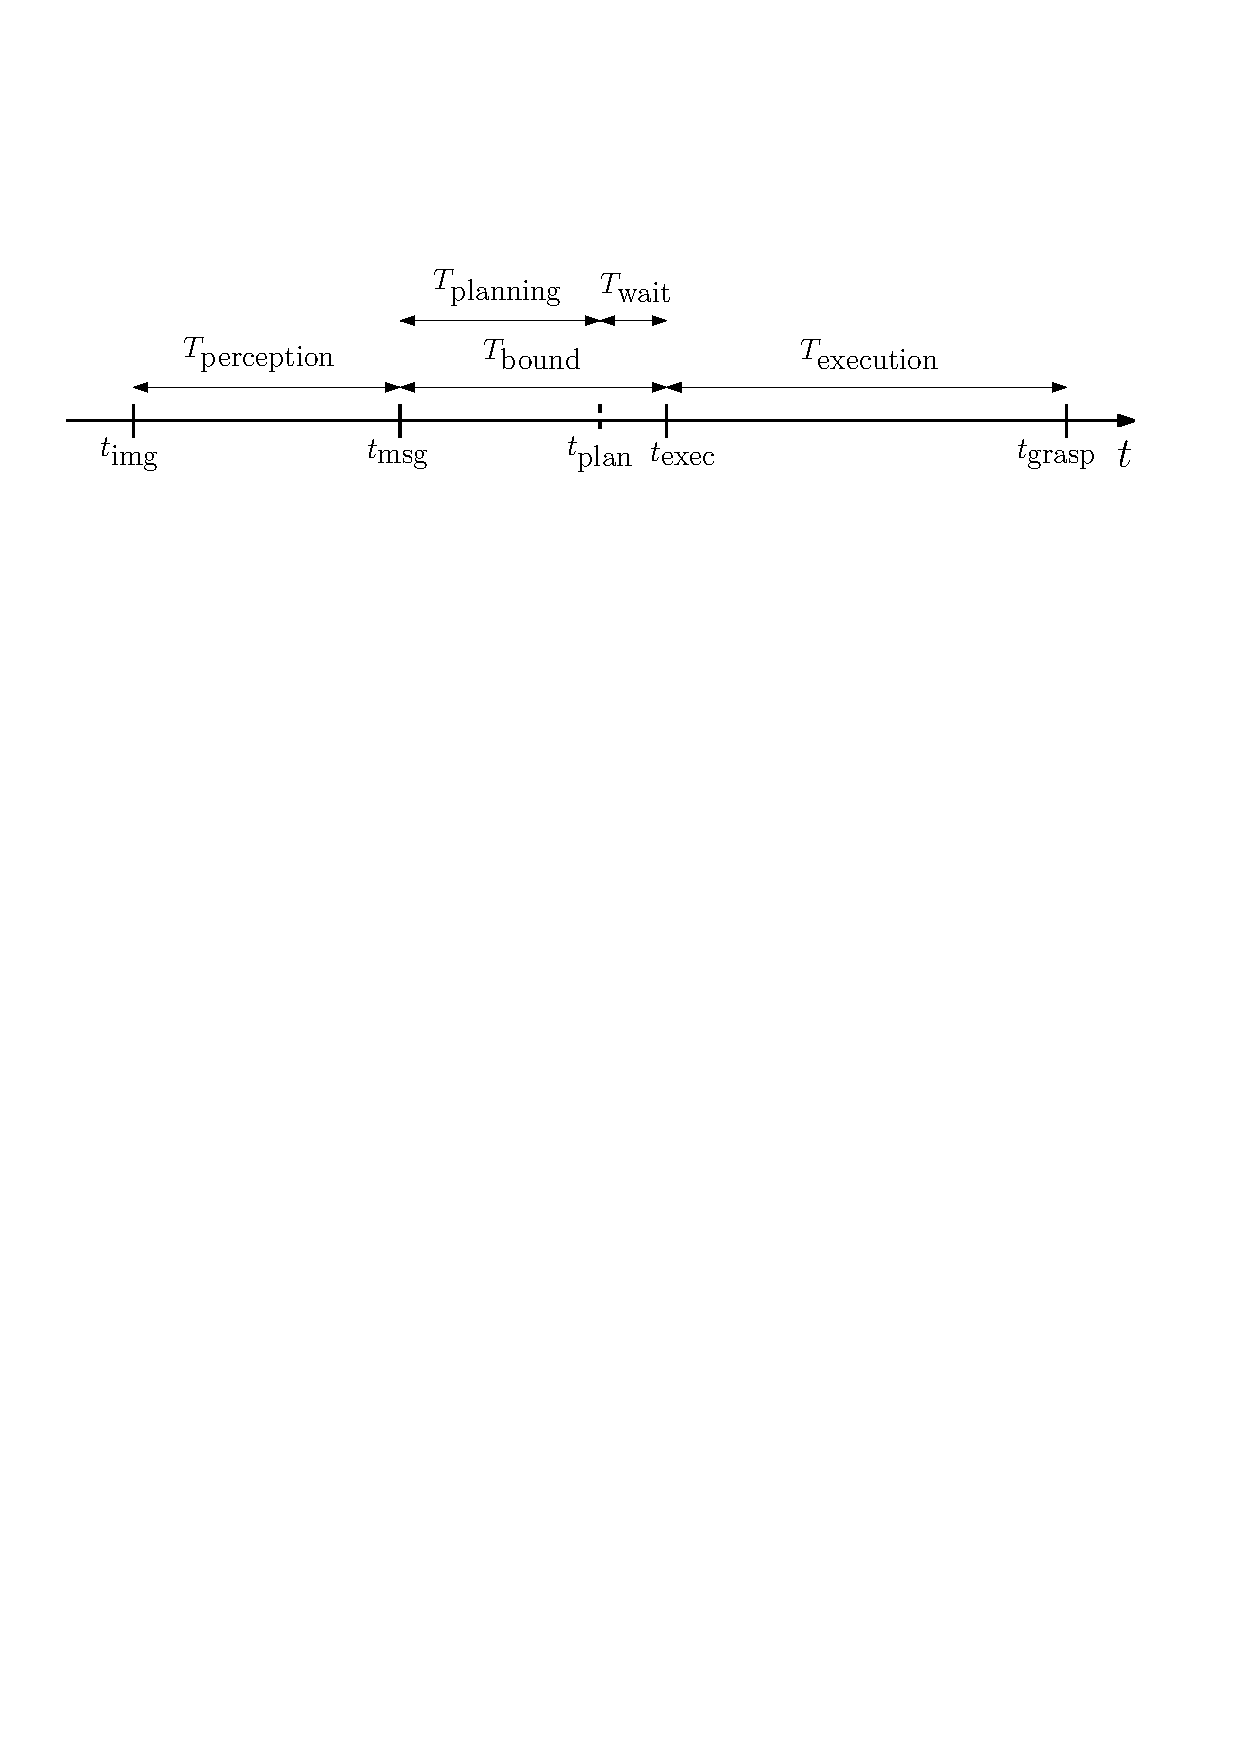
\includegraphics[width=0.5\textwidth]{figs/timeline2.pdf}
    \caption{\CaptionTextSize Timeline of the sense-plan-act cycle.}
    \label{fig:tl}
    \vspace{-5mm}
\end{figure}

\subsubsection{Goal region specification}
To define the set of all goal poses~$\Gfull$, we need to detail our system setup, depicted in Fig.~\ref{fig:pe}.
The conveyor belt $\calB$ moves along the $x$-axis from left to right.
We pick a fixed $x$-value termed~\Xexec, such that when the incoming $o$ reaches \Xexec as per the perception information, at that point we start execution.

% We assume that there exists a specific $x$-value, termed~\Xexec, such that when the robot start's executing for the first time, the object's  $x$-value will be in the range $[\Xexec-\varepsilon_\calP, \Xexec]$.
%any forward propagation to $t_{\rm exec}$ time an initial pose estimate is given for an object, its $x$-value is in the range $[\Xexec-\varepsilon_\calP, \Xexec]$.
%
Recall that a pose of an object~$o$ is a three dimensional point~$(x,y,\theta)$ corresponding to the $(x,y)$ location of~$o$ and to its orientation (yaw angle) along $\calB$.
%
$\Gfull$ contains a fine discretization of all possible $y$ and $\theta$ values and $x$ values in  $[\Xexec-\varepsilon_\calP, \Xexec+\varepsilon_\calP]$.
We select $\Gfull$ such that $\varepsilon_\calP = 0.5$ cm, dimension along $y$-axis is 20 cm. The discretization in $x,y$ and $\theta$ is 1.0 cm and 10 degrees respectively.

In the example depicted in Fig.~\ref{fig:pe}, the thick and the thin solid rectangles show the ground truth and estimated poses, respectively at two time instances in the life time of the object.
%
The first plan is generated for the pose shown at $x_{\textrm{exec}}$. During execution, the robot receives an improved estimate and has to replan for it. At this point we back project this new estimate in time using the known speed of the conveyor and the time duration between the two estimates. This back-projected pose (shown as the dotted rectangle) is then picked as the new goal for replanning. Recall that under the assumption ~\ref{assum:3} the back projected pose will always lie inside \Gfull.
%
%Recall that we assume that the new estimate will be within the $\pm \varepsilon_\calP$ window around \Xexec, it will always lie within \Gfull. 
%As \Gfull contains all $y$ and $\theta$ values (up to our discretization), our system can handle the errors along those dimensions.



\begin{figure}
    \centering
    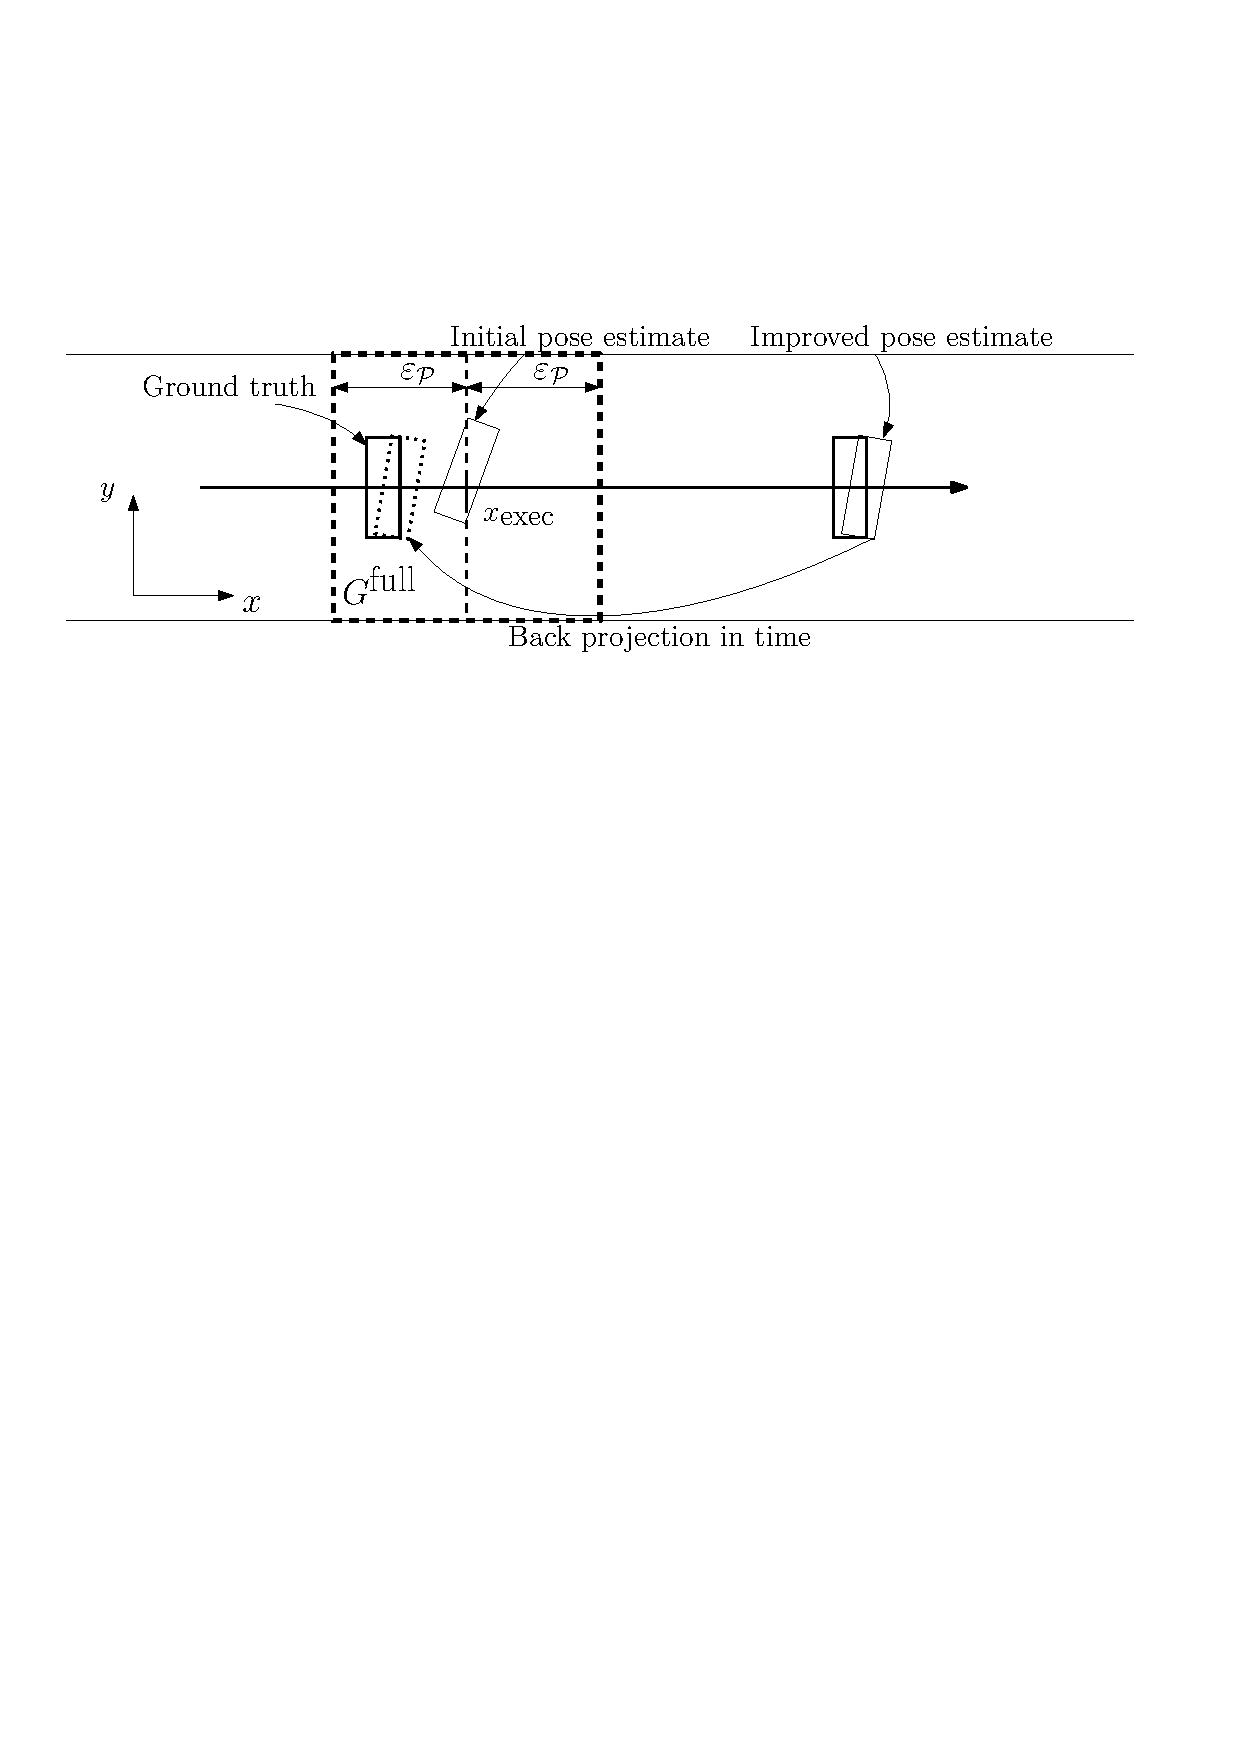
\includegraphics[width=0.5\textwidth]{figs/pose_error2.pdf}
    \caption{\CaptionTextSize A depiction of \Gfull-specification on a conveyor belt (overhead view) and perception noise handling. 
    }
    \label{fig:pe}
%        \vspace{-5mm}
\end{figure}

\subsection{Results}

Before we report on our system-level results comparing our work with alternative implementation (namely, results from the query stage), we mention that the preprocessing stage took roughly 3.5 hours and the memory footprint following this stage is less than 20 MB.
%
This backs up our intuition that the domain allows for efficient compression of a massive amount of paths in a reasonable amount of preprocessing time. In all experiments, we used $\Trc =3.5$ seconds




\subsubsection{Real-robot experiments}
\label{sec:robot_results}
To show the necessity of real-time replanning we performed three types of experiments, 
(E1)~replanning with multiple pose estimates, 
(E2)~first-pose planning from the first object pose estimate 
%(received at approximately 1.5m from the robot's base) 
(E3)~best-pose planning from the late (more accurate) pose estimate. 
%
For each set of experiments, we determined the pickup success rate to grasp the moving object (sugar box) off~$\calB$. In addition, we report on $\calP$'s success rate by observing the overlap between the point cloud of the object's 3D model transformed by the predicted pose (that was used for planning) and the filtered input point cloud containing points belonging to the object. 
A high (resp. low) overlap results in an accurate (resp. inaccurate) pose estimate. 
%
We use the same strategy to determine a range for which $\calP$'s estimates are accurate and use it for best-pose planning. 
%This range is found to be 1.05m to 0.95m from the robot's base on the conveyor. 
Further, for each method, we determine the pickup success rate given that the perception was or wasn't accurate. 

The experimental results are shown in Table \ref{tab:robot_results}. Our method achieves the highest overall pickup success rate on the robot, indicating the importance of continuous replanning with multiple pose estimates. 
First-pose planning has the least overall success rate due to inaccuracy of pose estimates when the object is far from the robot's camera. 
Best-pose planning performs better overall than the first pose strategy, since it uses accurate pose estimates, received when the object is close to the robot. However it often fails even when perception is accurate, due to the limited time remaining to grasp object when it's closer to the robot. 
%We can observe this from the method's lowest pickup success rate among the 3 methods when perception = 1 in \ref{tab:robot_results}.






\begin{table}[t]
\centering
\begin{tabular}{|c|c|c|c|c|}
\hline
                    & \begin{tabular}[c]{@{}c@{}}Overall \\ Pickup\end{tabular}
                    & Perception 
                    & \begin{tabular}[c]{@{}c@{}}Pickup \\ (Perception = 1*)\end{tabular} 
                    & \begin{tabular}[c]{@{}c@{}}Pickup \\ (Perception = 0*)\end{tabular} \\ \hline
E1          & \textbf{69.23}                                                                      & \textbf{42.31}                   & \textbf{83.33}                                                                             & \textbf{57.14}                                                                             \\ \hline
E2 & 16.00                                                                      & 24.00                   & 66.67                                                                             & 0.00                                                                              \\ \hline
E3   & 34.61                                                                      & 34.62                   & 55.56                                                                             & 23.53                                                                             \\ \hline
\end{tabular}
\caption{\CaptionTextSize Real-robot experiments. Success rate for the three experiments (E1---our method, E2---First-pose planning and E3---Best-pose planning). Perception = 1 is accurate estimate, Perception = 0 is inaccurate}
\label{tab:robot_results}
\vspace{-5mm}
\end{table}

\ignore{
\begin{table*}[t]
\centering
\begin{tabular}{|c|c|c|c|c|}
\hline
                    & \begin{tabular}[c]{@{}c@{}}Pickup success rate [\%]\\ (Overall)\end{tabular} & Perception success rate [\%]& \begin{tabular}[c]{@{}c@{}}Pickup success rate [\%]\\ (Perception = 1*)\end{tabular} & \begin{tabular}[c]{@{}c@{}}Pickup success rate [\%]\\ (Perception = 0*)\end{tabular} \\ \hline
Our method (E1)          & \textbf{9.23}                                                                      & \textbf{42.31}                   & \textbf{83.33}                                                                             & \textbf{57.14}                                                                             \\ \hline
First-pose planning (E2) & 16.00                                                                      & 24.00                   & 66.67                                                                             & 0.00                                                                              \\ \hline
Best-pose planing (E3)   & 34.61                                                                      & 34.62                   & 55.56                                                                             & 23.53                                                                             \\ \hline
\end{tabular}
\caption{Real-robot Experiments}
\label{tab:robot_results}
\end{table*}
}

\subsubsection{Simulation experiments}






We simulated the real world scenario to evaluate our method against other baselines. We compared our method with \wastar, \textsc{E-graphs} and \rrt. 
For \wastar and \textsc{E-graphs} we use the same graph representation as our method. 
For \textsc{E-graphs} we precompute five paths to randomly-selected  goals in \Gfull. 
We adapt the \rrt algorithm to account for the under-defined goals. To do so, we sample pre-grasp poses along the conveyor 
%in the reachable workspace with a fine discretization 
and compute IK solutions for them to get a set of goal configurations for goal biasing. 
When a newly-added node falls within a threshold distance from the object, we use the same dynamic primitive that we use in the search-based methods to add the final grasping maneuver. If the primitive succeeds, we return success. We also allow wait actions at the pre-grasp locations.

For any planner to be used in our system, we need to endow it with a (possibly arbitrary) planning time bound to compute the future location of the object from which the new execution will start (see Fig.~\ref{fig:tl}). 
%
If the planner fails to generate the plan within this time, then the robot misses the object for that cycle and such cases are recorded as failures. 
%
We label a run as a ``Pickup success" if the planner successfully replans once after the object crosses the 1.0m mark. The mark is the mean of accurate perception range that was determined experimentally and used in the robot experiments as described in Section \ref{sec:robot_results}.
%
The key takeaway from our experiments (Table~\ref{tab:sim_results}) is that having a known time bound on the query time is vital to the success of the conveyor pickup task.

Our method shows the highest pickup success rate, planning success rate (success rate over all planning queries) and an order of magnitude lower planning times compared to the other methods. 
The planning success rate being lower than 100\% can be attributed to the fact that some goals were unreachable during the runs. 
%
We tested the other methods with several different time bounds. Besides our approach \textsc{E-graphs} perform significantly well. \rrt suffers from the fact that the goal is under-defined and sampling based planners typically require a goal bias in the configuration space. Another important highlight of the experiments is the number of planning cycles over the lifetime of an object. While the other approaches could replan at most twice, our method was able to replan thrice due to fast planning times.


\ignore{
\begin{table*}[t]
\centering
\begin{tabular}{|c||c||c|c|c||c|c|c||c|c|c|}
\hline
   & \textbf{Our Method} 
   & \multicolumn{3}{c|}{\wastar}
   & \multicolumn{3}{c|}{\textsf{E-Graph}}
   & \multicolumn{3}{c|}{\rrt}
   \\ \hline
   & $T_{b}$ = 0.2 
   & $T_{b}$ = 0.5 & $T_{b}$ = 1.0 & $T_{b}$ = 2.0 
   & $T_{b}$ = 0.5 & $T_{b}$ = 1.0 & $T_{b}$ = 2.0 
   & $T_{b}$ = 0.5 & $T_{b}$ = 1.0 & $T_{b}$ = 2.0 
   \\ \hline
Pickup success rate [\%]                   & 92.00     & 0.00      & 0.00     & 18.00      & 0.00        & 0.00       & 80.00       & 0.00       & 0.00       & 18.00      \\ \hline
Planning success rate [\%]                  & 94.67     & 4.00       & 17.00      & 19.00       & 31.00    & 80.00       & 90.00      & 12.00      & 9.00       & 13.00       \\ \hline
Planning time [s]                    & 0.0689       & 0.4329        & 0.6284        & 0.8241        & 0.2830        & 0.4194        & 0.3112        & 0.2718        & 0.2518        & 0.1966        \\ \hline
Planning episodes per pickup & 3            & 2             & 2             & 2             & 2             & 2             & 2             & 2             & 2             & 2             \\ \hline
Path cost [s]                         & 10.11        & 8.19          & 8.28          & 7.60          & 8.54          & 8.22          & 7.90          & 9.68          & 8.96          & 8.04          \\ \hline
%Expansions                        & 17.57        & 315.50        & 392.81        & 495.78        & 188.24        & 202.63        & 137.02        & 146.54        & 104.75        & 78.64         \\ \hline
\end{tabular}
\caption{Simulation results. Here $T_b$ denotes the (possibly arbitrary) timbound that the algorithm uses. Note that for our method $T_b = \Tbound$ is the time bound that the algorithm is ensured to compute a plan.}
\label{tab:sim_results}
\end{table*}
}


% \begin{table}[t]
% % \centering
%     \resizebox{0.5\textwidth}{!}{ 
%         \begin{tabular}{ l | c c c c}
%           & \algname{WA*} & \algname{E-graphs} & \algname{\rrt} & \textbf{Our method} \\
%          \hline
%          Planning time [ms]& - (-) & - (-) & - (-) & \textbf{- (-)}\\
%          Success rate [$\%$]& - & - & - & \textbf{-}\\
%          No. of replans& - & - & - & \textbf{-}\\
%         \end{tabular}
%     }
%     \caption{Planning times, success rate and number of replanning queries averaged over 100 simulated runs of an object moving on $\calB$.}
%     \label{tab:stats_query}
% \end{table}


\ignore{
\begin{figure}
    \centering
    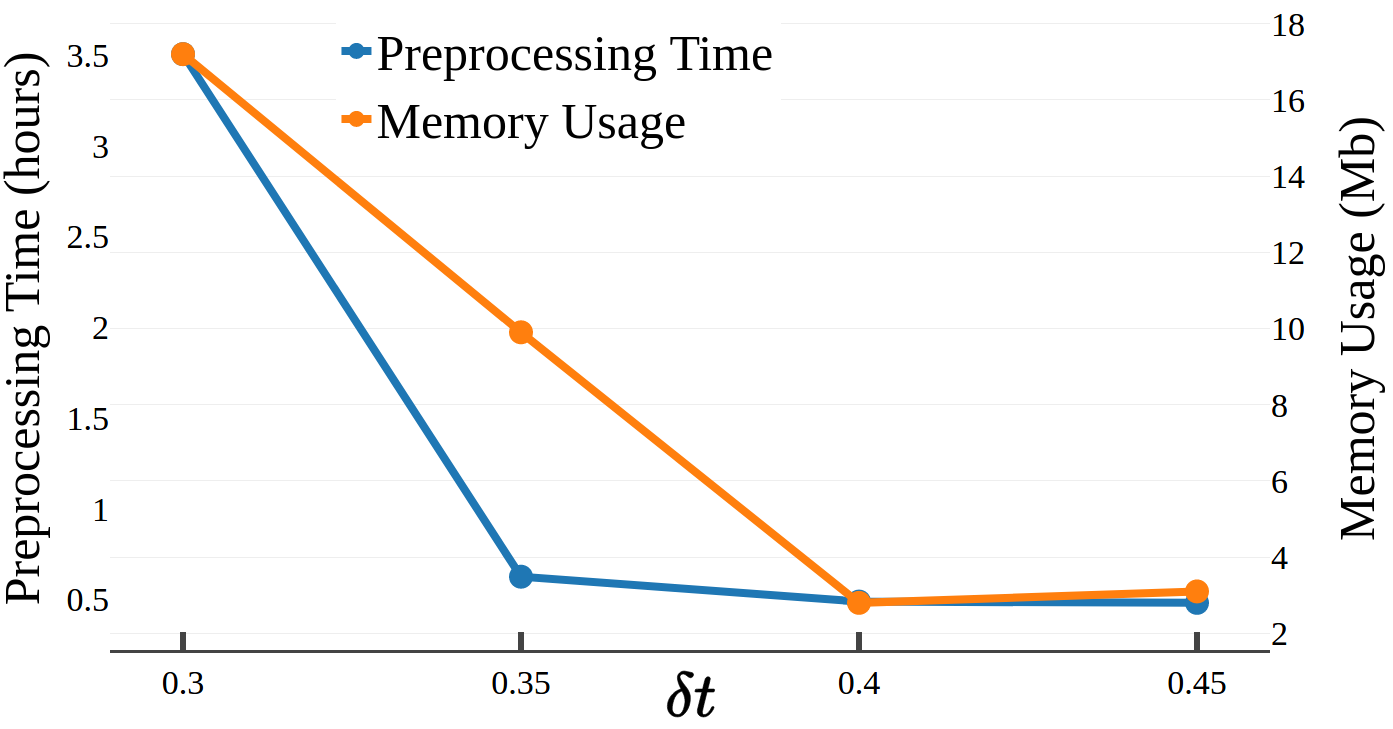
\includegraphics[width=0.4\textwidth]{figs/preprocess.png}
    \caption{Preprocessing}
    \label{fig:preprocessing}
\end{figure}
}


%\section{Conclusion \& future work}

%\section*{Acknowledgments}


%% Use plainnat to work nicely with natbib. 

\newpage
\bibliographystyle{plainnat}
\bibliography{references}

\end{document}


